\chapter{Items and Equipment}

This chapter defines the items and equipment that exist in the universe of Rise, including both magical and nonmagical items.

\section{Wealth and Item Ranks}\label{Wealth}\label{Wealth and Item Ranks}

  The worth of an item can be measured with money, or with the more abstract concept of an item's rank.
  Both measurements are closely connected.
  In general, gold pieces are a more useful concept at low levels, and item rank are more useful at high levels.
  However, both concepts function at any level, so you can use whichever makes more sense in a particular game.

  \subsection{Coins}
    Most common people would use the silver piece (sp) for daily usage, with copper pieces (cp) used for change and trivial matters.
    However, adventurers and nobility typically deal with the gold piece (gp).
    A gold piece is worth 100 silver pieces, and a silver piece is worth 100 copper pieces.

    The standard coin weighs about a third of an ounce (fifty to the pound).

    \begin{dtable}
      \lcaption{Coin Exchange Values}
      \begin{dtabularx}{\columnwidth}{l c *{3}{>{\ccol}X}}
        &   & \tb{CP} & \tb{SP} & \tb{GP} \tableheaderrule
        Copper piece (cp)   & = & 1      & 1/100 & 1/10,000 \\
        Silver piece (sp)   & = & 100    & 1     & 1/100    \\
        Gold piece (gp)     & = & 10,000 & 100   & 1        \\
      \end{dtabularx}
    \end{dtable}

  \subsection{Item Ranks}\label{Item Ranks}

    % Consumable items get effects at +1 rank, since they are cheap.
    Each item has a rank associated with it.
    An item's rank is generally correlated with the item's effectiveness, rarity, and value.
    A magic item's \glossterm{power} is equal to twice its rank.
    In general, five items of a given rank are worth the same as a single item that is one rank higher.
    These effects are summarized in Item Ranks, below.

    \begin{columntable}
      \begin{dtabularx}{\columnwidth}{l l X}
        \tb{Rank} & \tb{Typical Item Price} & \tb{Power} \tableheaderrule
        0         & 1 gp or less            & 0  \\
        1         & 4 gp                    & 2  \\
        2         & 20 gp                   & 4  \\
        3         & 100 gp                  & 6  \\
        4         & 500 gp                  & 8  \\
        5         & 2,500 gp                & 10 \\
        6         & 12,500 gp               & 12 \\
        7         & 62,500 gp               & 14 \\
        8         & 312,500 gp              & 16 \\
      \end{dtabularx}
    \end{columntable}

    Items with a rank of 0 or 1 may be found among common folk, though few commoners would have more than one magic item of any value.
    Items with a rank of 2 or higher are usually only owned or used by nobility, wealthy merchants, and adventurers.

  \subsection{Buying and Selling Items}
    Items of any rank can be exchanged for other items based on their rank.
    In general, items with an rank of 3 or less can be bought or sold in exchange for gold pieces.
    Items with an rank of 4 or higher are exceptionally rare.
    The monetary value of such items is so exorbitant that they are almost never purchased or sold with gold pieces.
    Instead, they are typically exchanged for similarly rare magic items or gems.

    Wandering adventurers typically have a limited time frame to sell their items.
    It can be difficult to find a buyer for valuable items on short notice, so they must accept lower prices than merchants can charge.
    When selling for gold pieces, you can expect to receive a fifth of the item's typical value according to its rank.
    When selling for another item, you can expect to receive an item or trade good of one rank lower in exchange.
    These ratios can be negotiated, and favorably disposed merchants or nobles may give better deals.

    Some items have no listed price, such as arrows.
    They are not literally free in-universe, but the price of those items is typically not meaningful to track.
    If it's relevant, their price should generally be measured in silver pieces, at the GM's discretion.

    \subsubsection{Trade Goods}
      Some items are considered trade goods.
      Trade goods have a widely agreed upon value, but no intrinsic use.
      Gold pieces and gems are examples of trade goods.
      Trade goods differ from other items in that even adventurers can typically receive their full value when selling them to established merchants.
      Some common trade goods are detailed in \tref{Trade Goods}.

      \begin{dtable}
        \lcaption{Trade Goods}
        \begin{dtabularx}{\columnwidth}{l >{\lcol}X}
          \tb{Cost} & \tb{Item} \tableheaderrule
          10 cp & One pound of wheat \\
          20 cp & One pound of flour \\
          1 sp & One pound of iron, or one chicken \\
          5 sp & One pound of tobacco or copper \\
          10 sp & One pound of cinnamon, or one goat \\
          20 sp & One pound of ginger or pepper, or one sheep \\
          30 sp & One pig \\
          40 sp & One square yard of linen \\
          50 sp & One pound of salt or silver \\
          1 gp & One square yard of silk, or one cow \\
          2 gp & One pound of saffron or cloves, or one ox \\
        \end{dtabularx}
      \end{dtable}

  \subsection{Typical Wealth Acquisition}
    A typical character finds one non-consumable item appropriate for them per level.
    That item would have a rank equal to that character's highest rank at the time.
    For example, a typical 5th level character would have five items: two rank 2 items, and 3 rank 1 items.
    In addition, characters typically find several consumable items per level that are appropriate to their rank.

    Over time, lower rank items stop being useful, so most characters use no more than five or six different items at a time, plus various consumables.
    A typical 20th level character does not carry around 20 different items.
    However, the lower level items are essentially irrelevant from the perspective of calculating wealth, so the ``one item per level'' guideline is still useful.

    This is a drastic simplification of the sometimes messy process of accumulating wealth and magic items over the course of a typical campaign.
    Characters will often find additional items that they have no immediate use for.
    Players may go several sessions without acquiring any particular items until they complete their current quest, which may reward them with a large number of items at once.
    This is all fine, and the GM should not feel compelled to keep item acquisition perfectly on rails.
    Rise is only loosely balanced around this general pace of item acquisition, and it is not hard - or always necessary - to adjust encounters to deal with unusually wealthy or poor characters.

\section{Using Items}

  \subsection{Manipulating Objects}\label{Manipulating Objects}
    There are two ways to determine how difficult an object is to interact with: its weight, and how it is contained.
    Use the slowest action type from among the both methods.
    Some objects have special rules that indicate how much time they take to interact with, such as \weapontag{Heavy} weapons.
    Those rules override these general guidelines.

    You can only manipulate objects as a free action once per round.
    However, you can use a minor action or a standard action in place of a free action for this purpose, allowing you to manipulate up to three objects per round.
    These object manipulation rules are intended to cover interactions that take some amount of time and effort, such as drawing a weapon or opening a door.
    Simply dropping an object in your hands is so trivial that it does not count against your one free action object manipulation per round.
    Other similarly simple interactions may not count against that limit at the GM's discretion.

    \begin{raggeditemize}
      \itemhead{Containment} If the item is freely accessible, interacting with that item is a \glossterm{free action}.
        Drawing or sheathing an item from a dedicated container for that item, such as a weapon sheath, is normally a \glossterm{minor action}.
        Withdrawing an item from a disorganized heap, such as a bag or backpack, requires a \glossterm{standard action}.
      \itemhead{Weight} If an item's weight category is no heavier than your \glossterm{carrying capacity}, interacting with that item is a \glossterm{free action} (see \pcref{Weight Limits}).
        Pushing or dragging something that exceeds your carrying capacity requires a \glossterm{standard action}.
    \end{raggeditemize}

  \subsection{Moving Items Between Hands}\label{Moving Items Between Hands}
    In general, you can move weapons and similar handheld objects between your hands without using an action, as long as you are strong enough to hold their combined weight in one hand.
    For example, if you were holding two short swords, you could quickly hold them both in one hand to open a door or cast a spell, and then return to holding one in each hand.
    Likewise, you can reload a longbow without worrying about when you are holding the longbow (and string) with both hands or holding it in one hand while retrieving an arrow from a quiver with the other hand.
    Since shields are more cumbersome to don and remove, this does not allow you to use your shield hand as a free hand in the same way.

  \subsection{Storing Items}\label{Storing Items}
    A character can only store a limited number of weapons in locations that are easy to access in combat.
    Generally, a humanoid creature can carry no more than five ordinary weapons or shields on their body.
    For each additional weapon or similar item stored in a convenient location, you increase your \glossterm{encumbrance} by 1.
    Items carried outside of easy reach in combat, such as in a backpack, are ignored for this purpose.

    A Heavy weapon takes up twice the space of an ordinary weapon, and a Light weapon takes up half that space.
    Compact weapons do not take up a meaningful amount of space, and can be ignored for this purpose.
    Ammunition is typically stored in a quiver or pouch.
    Treat ammunition storage as a separate Light item that can hold an unlimited quantity of any ammunition other than lances.

    For example, you could carry up to ten Light weapons, four normal weapons and a standard shield, or two Heavy weapons plus a normal weapon.

  \subsection{Magic Item Activation}

    Some magic items have to be explicitly activated to have unusual effects.
    For example, the \mitem{seven league boots} can be activated to teleport you across great distances.
    Other magic items constantly have magical effects.
    For example, a \mitem{ring of protection} passively grants you a defense bonus.

    The description of a magic item effect will specify what mechanical actions must be taken, if any, to activate the effects of the item.
    For example, a belt of healing requires a \glossterm{standard action} to activate.
    However, the item description will not specify the exact nature of the action.
    Different items, even if they have the same effect, can have different physical actions that are required to activate the item.
    These activation actions can come in one of the following forms:
    \begin{itemize}
      \item Command word: You must speak a specific word that the item will hear and react to.
        For example, you may need to say the word ``healing'' in Elven to activate an item that heals you.
      \item Mental command: You must mentally direct the item to activate, such as by visualizing the item or thinking a particular word.
        % TODO: does this item exist
        For example, you may need to imagine a warm blanket around you to activate an item that protects you from cold damage or environmental effects.
      \item Physical motion: You must perform a specific physical motion, usually involving the item in some way.
        For example, you may need to rapidly stomp one foot on the ground to activate an item that allows you to move faster.
    \end{itemize}

    % TODO: table of random item activations?

  \subsection{Magic Item Limitations}

    There are three restrictions on your ability to use magic items.
    First, you cannot equip two apparel items that take up the same physical location on your body.
    For example, you cannot equip two different gauntlet sets and gain the effects of both, but you could equip several amulets or up to ten rings.

    Second, all magic items require you to attune to them to gain their effect unless they indicate otherwise in their description.
    You can attune to a magic item with the \textit{item attunement} ability, below.

    Third, you cannot attune to two items with the same name, or if one is simply an upgrade of another one.

    \subsubsection{Item Attunement}\label{Item Attunement}

      As a standard action, you can use the \textit{item attunement} ability to attune to items.
      This is a \magical ability.

      \begin{attuneability}{Item Attunement}{\abilitytag{Attune}}
        \abilityusagetime Standard action.
        \rankline
        Choose a magic item you are touching.
        Any abilities the target has that require attunement become active, allowing you to use its full potential.
      \end{attuneability}

      \parhead{Shared Item Attunement} Multiple creatures can attune to the same item simultaneously.
      Since most items only function while worn or wielded, this does not usually allow multiple creatures to gain the benefits of the item.
      However, the creatures can swap the item between them without having to reattune to it each time.

    \subsubsection{Magic Item Power}\label{Magic Item Power}
      The \glossterm{power} of an item is equal to twice its rank.
      An item's power also affects its defenses.
      Its Fortitude and Mental defenses are equal to 5 \add its \glossterm{power}.
      % TODO: how are those determined?
      Its Armor, Brawn, and Reflex defenses are not affected by its \glossterm{power}, and are solely determined by its size and shape.

  \subsection{Removing Magic Items}
    Unless otherwise noted, magic items that have effects on the creature using the item must continue to be worn or held as long as the effect lasts.
    If a magic item has an ability with a duration, removing the item also ends the ability.
    Items which are consumed when used or which do not affect their user are unaffected by this rule.

\newpage
\sectiongraphic*{Weapons}{width=\columnwidth}{equipment/weapons}

  Each weapon has a \glossterm{weapon group} and any number of \glossterm{weapon tags}.
  In addition, each weapon has a particular \glossterm{accuracy} modifier and defines a base \glossterm{dice pool} for attacks using that weapon.
  This section explains each of those concepts and defines the statistics for weapons in Rise.
  You gain a bonus to your \glossterm{weapon damage} equal to half your \glossterm{power} (see \pcref{Weapon Damage}).

  Unless otherwise specified, a weapon must be held in a single \glossterm{free hand}.
  You can use two hands to hold a weapon if you want, but that provides no special benefit unless that weapon has the \weapontag{Versatile Grip} tag (see \pcref{Weapon Tags}).

  \subsection{Weapon Groups}\label{Weapon Groups}
    Weapons are organized into thematically related categories called weapon groups. They are described in \trefnp{Weapon Groups}. For example, all axes belong to the ``axes'' weapon group. Some weapons can be found in multiple weapon groups. For example, a dagger is a simple weapon, a blade, and a thrown weapon.

    \parhead{Exotic Weapons}\nonsectionlabel{Exotic Weapons} Some weapons are rare and have unusual fighting styles.
    These weapons are called exotic weapons.
    Although many characters are proficient with non-exotic weapons, proficiency with exotic weapons is rare.
    Some specific class abilities grant proficiency with exotic weapons.

    \begin{dtable!*}
      \lcaption{Weapon Groups}
      \begin{dtabularx}{\textwidth}{l >{\lcol}X >{\lcol}X}
        \tb{Group}         & \tb{Weapons}                                                                & \tb{Exotic Weapons} \tableheaderrule
        Armor weapons      & Standard shield, spiked shield                                              & Armblade, spiked knee                                            \\
        Axes               & Battleaxe, greataxe, handaxe, poleaxe, shepherd's axe, throwing axe         & Dwarven throwing axe, dwarven waraxe, orcish greataxe            \\
        Blades             & Broadsword, dagger, greatsword, rapier, scimitar, smallsword                & Boot dagger, falchion, katana, kukri                             \\
        Bows               & Longbow, shortbow                                                           & Flatbow, heartseeker arrows, recurve bow, takedown bow, titanbow \\
        Club-like weapons  & Club, greatmace, mace, morning star, sap, torch                             & Culacula, gnomish trick mace, knobkerrie, totokia                \\
        Crossbows          & Heavy crossbow, light crossbow, pellet crossbow                             & Arbalest, pistol crossbow, repeating crossbow   \\
        Flexible Weapons   & Flail, heavy flail, nunchaku, two-section staff, whip                       & Chain whip, meteor hammer, three-section staff                   \\
        Headed weapons     & Light hammer, longhammer, pick, sickle, sledgehammer, warhammer             & Dwarven longhammer, dwarven shorthammer, heavy pick, obuch       \\
        Improvised weapons & \tdash                                                                      & \tdash                                                           \\
        Monk weapons       & Jitte, kama, kunai, nunchaku, quarterstaff, shuriken, two-section staff     & Hook sword, sai, three-section staff, war fan                    \\
        Polearms           & Bardiche, glaive, halberd, longhammer, poleaxe, quarterstaff, scythe        & Fauchard, war scythe                                             \\
        Simple weapons     & Club, dagger, mace, quarterstaff                                            & \tdash                                                           \\
        Spears             & Greatspear, javelin, spear, spontoon                                        & Cavalry lance, gnomish smallspear, partisan, pike                               \\
        Thrown weapons     & Dagger, dart, handaxe, javelin, light hammer, shuriken, sling, throwing axe & Dwarven throwing axe, dwarven waraxe, net                 \\
      \end{dtabularx}
    \end{dtable!*}

    \subsubsection{Weapon Proficiency}\label{Weapon Proficiency}
      You take a \minus2 accuracy penalty with weapons you are not proficient with.

    \subsubsection{Improvised Weapons}\label{Improvised Weapons}
      Sometimes objects not crafted to be weapons nonetheless see use in combat.
      In general, treat improvised weapons as being equivalent to the non-exotic manufactured weapon that seems most similar in shape and composition.
      However, since you are not proficient with the improvised weapon, you take a \minus2 accuracy penalty with it.
      If you become proficient with improvised weapons, this accuracy penalty is removed.

    \subsubsection{Natural Weapons}\label{Natural Weapons}
      Natural weapons are weapons that are part of a creature's body instead of being manufactured and wielded.
      Many monsters have natural weapons, like claws or a bite attack.
      Natural weapons do not normally require a \glossterm{free hand} to use.
      All bipedal creatures also have two punch/kick natural weapons.

      Common natural weapons are listed in \tref{Natural Weapons}.
      In addition, some monsters and effects have unique natural weapons, such as the \spell{stonefist} spell.

      \parhead{Physical Size} Like all objects and creatures, weapons have a size category that represents how physically large they are. Most weapons are one size category smaller than their wielder, but \weapontag{Heavy} weapons are the same size category as the wielder.
      All weapons are \glossterm{lightweight} unless otherwise noted.

      \parhead{Inappropriately Sized Weapons}\nonsectionlabel{Inappropriately Sized Weapons} You can use weapons that are sized for creatures that are one size category larger or smaller than you.
      However, you take a \minus2 accuracy penalty on attacks using an inappropriately sized weapon.

  \subsection{Weapon Range Limits}\label{Weapon Range Limits}
    Ranged weapon attacks become less accurate if the target is far away.
    Ranged weapons have two \glossterm{range limits} listed, with a slash between them, such as 90/270.
    The first number indicates the maximum range for a weapon's \glossterm{close range}.
    The second number indicates the maximum range for a weapon's \glossterm{long range}.
    You cannot attack a target that is beyond a weapon's long range limit.

    Attacks at close range have no penalty.
    Attacks at long range have a \minus4 accuracy penalty.
    This is called a \glossterm{longshot penalty}, and some abilities can reduce this penalty.

  \subsection{Weapon Tags}\label{Weapon Tags}
    Some weapons found on \trefnp{Weapons} have tags that indicate that they have special abilities. The list of abilities that weapons can have is given below.
    \weapontagdef{Ammunition} When you hit with a strike using this weapon, it becomes \glossterm{broken}.
    It cannot have magic weapon properties.
    However, whenever you buy or craft this weapon, you receive multiple copies, as indicated in the table below.
    \weapontagdef{Bow} This weapon is a bow used to fire arrows.
    You need both hands to fire a bow.
    Drawing an arrow from a quiver and notching it into a bow requires one \glossterm{free hand} while holding the bow in another hand.
    This is not considered an independent action, so you can fire a bow any number of times per round.
    \weapontagdef{Clinch} You gain a \plus2 bonus to \glossterm{accuracy} on \glossterm{melee} \glossterm{strikes} using this weapon against creatures who are \grappled.
    \weapontagdef{Compact} This weapon is unusually small.
    It is one size category smaller than normal (that is, two size categories smaller than the creature it is intended for).
    This makes it easier to conceal (see \pcref{Sleight of Hand}).
    In addition, you only take a \minus5 penalty to Stealth when trying to conceal strikes with a Compact weapon instead of the normal \minus10 or \minus20 penalty for concealing a strike (see \pcref{Stealth}).
    \weapontagdef{Heavy} Heavy weapons are larger and heavier than other weapons.
    You normally need two hands to use a Heavy weapon, whether you are throwing it or using it in melee.
    Drawing a Heavy item from a sheath, or returning it to a sheath, requires a \glossterm{standard action}.

    If you have a Strength of 3 or higher, you draw or sheathe a Heavy item at the same speed as non-Heavy items.
    In addition, you can wield a Heavy weapon in one hand, but you take a \minus1 accuracy penalty with the weapon while doing so.
    This cannot be used if the weapon always requires two hands to fire, such as a titanbow.
    If your Strength is 6 or higher, this accuracy penalty is removed.

    While holding a Heavy weapon in two hands, you gain a \plus1 bonus per 3 \glossterm{power} to your \glossterm{weapon damage} with the weapon.
    This bonus is in addition to the normal bonus that you gain from your power with weapons (see \pcref{Weapon Damage}).
    \weapontagdef{Impact} You get a \glossterm{glancing blow} with this weapon when you would miss by 5 or less (see \pcref{Glancing Blows}).
    This does not allow you to get glancing blows if that would normally be impossible for you.
    % Assume you have a 70% chance to hit (+0 vs AD 4).
    % +3 accuracy takes you to 1x hit damage per round.
    % +6 accuracy for crits means you crit on 8/9/10.
    % That's a 40% chance for a regular hit, a 20% chance for a glancing blow, and a 30% chance for a crit, so 1.1x hit damage per round.
    % Therefore, +2 accuracy with crits is worth about +1 global accuracy.
    \weapontagdef{Keen} You gain a \plus2 bonus to \glossterm{accuracy} with \glossterm{strikes} using this weapon for the purpose of determining whether you get a \glossterm{critical hit}.
    \weapontagdef{Light} Light weapons are smaller and easier to handle than other weapons.
    Drawing a Light item from a sheath, or returning it to a sheath, is a \glossterm{free action} rather than a minor action (see \pcref{Manipulating Objects}).
    Attacking with two weapons at once is more accurate with Light weapons (see \pcref{Dual Strikes}).
    \weapontagdef{Long}\label{Long Weapon} This weapon can be used to make melee \glossterm{strikes} against targets up to 10 feet away from you.
    If you use an ability with more specific targets than simply making a melee strike, such as affecting ``all enemies adjacent to you'', this weapon tag does not increase your range with that ability.
    \weapontagdef{Maneuverable} Whenever you use a \atBrawling ability that would normally require a free hand, you can use this weapon instead of a free hand.
    This has no benefit other than removing the requirement for a free hand.
    % TODO: wording
    As a result, being \grappled does not prevent you from making \glossterm{strikes} using your hands that are holding Maneuverable weapons.
    \weapontagdef{Mounted}\label{Mounted Weapon} If you are mounted, and your mount moves in the same phase that you make a \glossterm{strike} with a Mounted weapon, you gain a \plus2 \glossterm{accuracy} bonus with the strike.
    \weapontagdef{Parrying} If a creature attacks you with a \glossterm{melee} \glossterm{strike} while you wield this weapon, you \glossterm{briefly} gain a \plus2 bonus to \glossterm{accuracy} with strikes using this weapon against that creature.
    \weapontagdef{Projectile} This weapon fires ammunition at range to deal damage.
    The ammunition generally breaks when used.
    Projectile weapons have two \glossterm{range limits} listed in their description (see \pcref{Weapon Range Limits}).
    They must be reloaded after being fired.
    The time required to reload a projectile weapon is given in the weapon description.
    You take a \minus4 accuracy penalty with Projectile weapons against creatures adjacent to you.
    While riding a moving mount, you take a \minus4 accuracy penalty with Projectile weapons, and your range limits are halved.
    \weapontagdef{Resonating} Whenever you damage a creature with a strike using this weapon, it \glossterm{briefly} takes a -2 penalty to its Armor defense against your attacks.
    Unlike most non-damage effects, this penalty applies if you get a \glossterm{glancing blow} with the strike as long as the creature takes damage.
    \weapontagdef{Subdual} This weapon deals \glossterm{subdual damage} (see \pcref{Subdual Damage}).
    % (30/60) is one improvement, (60/120) is two.
    \weapontagdef{Sweeping}\label{Sweeping} When you make a \glossterm{melee} \glossterm{strike} with this weapon, you may add additional targets to the strike.
    Each additional target must be a valid target for the strike, which typically means it must be adjacent to you.
    Sweeping weapons have a number that indicates the number of targets you can add, such as Sweeping (2).
    \weapontagdef{Thrown} This weapon is designed to be thrown to deal damage at range.
    Thrown weapons have two \glossterm{range limits} listed in their description (see \pcref{Weapon Range Limits}).
    Unless otherwise noted in a weapon's description, a throwing weapon can be used to attack in melee without penalty.
    % Doesn't cost an improvement slot; very situational
    \weapontagdef{Versatile Grip} This weapon is designed to be held in either one hand or two hands.
    While holding a Versatile Grip weapon in two hands, you gain a \plus1 bonus per 3 \glossterm{power} to your \glossterm{weapon damage} with the weapon, with a minimum bonus of \plus1.
    This bonus is in addition to the normal bonus that you gain from your power with weapons (see \pcref{Weapon Damage}).

  \subsection{Weapon Table}
    Here is the format for weapon entries in the Weapons table, below.

    \parhead{Accuracy} This number modifies your \glossterm{accuracy} with \glossterm{strikes} using the weapon.

    \parhead{Damage} This \glossterm{dice pool} indicates the damage dealt by the weapon on a hit.

    \parhead{Item Rank (Cost)} The first value indicates the \glossterm{item rank} of the item (see \pcref{Item Ranks}).
    The second value in parentheses indicates the average cost to buy the item.
    Items crafted for unusually large or small creatures are more expensive.
    For each size category larger or smaller than Medium, the item's rank increases by one, which increases its price.

    \parhead{Weapon Tags} Some weapons have special properties. See \pcref{Weapon Tags} for details.

    % All weapons should have two improvements over a ``baseline'' +0a/1d6 weapon with no properties.
    % The Light weapon tag comes with an invisible +1a/-1d modifier, so +1a/1d4 with one extra improvement.
    % The Heavy weapon tag does not cost a tag slot and comes with an invisible +1d modifier, so +0a/1d8 with two extra improvements.
    \begin{longcolumn}
      \begin{longtablewrapper}
        \tablebookmark{Weapons}{weapons}
        \RaggedRight
        \begin{longtable}{p{12em} l l l >{\lcol}p{24em}}
          \lcaption{Weapons}                                                                                                                                         \\
          \tb{Name}                         & \tb{Accuracy} & \tb{Damage} & \tb{Item Rank (Cost)}\fn{1} & \tb{Tags}                          \tableheaderrule
          Armor weapons                     &               &             &                             &                                             \\
          \tind Standard shield             & \plus0        & 1d6         & 0 (1 gp)                    & \tdash                                      \\
          \tind Spiked standard shield      & \plus0        & 1d8         & 0 (1 gp)                    & \tdash                                      \\

          Axes                              &               &             &                             &                                             \\
          \tind Battleaxe                   & \plus0        & 1d8         & 0 (1 gp)                    & Sweeping (1), Versatile Grip                \\
          \tind Greataxe                    & \plus0        & 1d10        & 0 (1 gp)                    & Heavy, Sweeping (1)                         \\
          \tind Handaxe                     & \plus1        & 1d4         & 0 (1 gp)                    & Light, Thrown (30/60)                       \\
          \tind Poleaxe                     & \plus1        & 1d8         & 0 (1 gp)                    & Heavy, Maneuverable                         \\
          \tind Shepherd's axe              & \plus0        & 1d8         & 0 (1 gp)                    & Long, Versatile Grip                        \\
          \tind Throwing axe                & \plus0        & 1d8         & 0 (1 gp)                    & Thrown (30/60)                              \\

          Blades                            &               &             &                             &                                             \\
          \tind Broadsword                  & \plus1        & 1d6         & 0 (1 gp)                    & Sweeping (1), Versatile Grip                \\
          % -1d for an extra tag
          \tind Dagger                      & \plus1        & 1d3         & 0 (1 gp)                    & Compact, Light, Thrown (30/60)              \\
          \tind Greatsword                  & \plus0        & 1d8         & 0 (1 gp)                    & Heavy, Sweeping (2)                         \\
          \tind Rapier                      & \plus1        & 1d4         & 0 (1 gp)                    & Keen, Light                                       \\
          \tind Scimitar                    & \plus1        & 1d6         & 0 (1 gp)                    & Mounted                                     \\
          \tind Smallsword                  & \plus2        & 1d4         & 0 (1 gp)                    & Light                                 \\

          Bows                              &               &             &                             &                                             \\
          \tind Longbow\fn{2}               & \plus0        & 1d6         & 1 (4 gp)                    & Bow, Projectile (90/270)                    \\
          \tind Shortbow\fn{2}              & \plus0        & 1d4         & 1 (4 gp)                    & Bow, Projectile (60/180)                    \\
          \tind Arrows (20)                 & \plus0        & \tdash      & \tdash                      & Ammunition                                  \\
          \tind Blunted arrows (20)         & \minus1       & \tdash      & \tdash                      & Ammunition, Subdual                         \\
          \tind Fire arrows (20)\fn{2}      & \tdash        & \tdash      & 1 (4 gp)                    & Ammunition, \atFire                         \\
          \tind Lightning arrows (20)\fn{2} & \tdash        & \tdash      & 2 (20 gp)                   & Ammunition, \atElectricity                  \\

          Club-like weapons                 &               &             &                             &                                             \\
          \tind Cavalry mace                & \plus0        & 1d8         & 0 (1 gp)                    & Mounted, Versatile Grip                     \\
          % only 1 improvement
          \tind Club                        & \plus0        & 1d8         & \tdash                      & Versatile Grip                              \\
          \tind Greatmace                   & \plus0        & 1d10        & 0 (1 gp)                    & Heavy, Impact                               \\
          % only 1 improvement
          \tind Mace                        & \plus0        & 1d6         & 0 (1 gp)                    & Impact                                      \\
          \tind Morning star                & \plus0        & 1d10        & 0 (1 gp)                    & Versatile Grip                              \\
          % -1d for 3 tags
          \tind Sap                         & \plus1        & 1d3         & 0 (1 gp)                    & Compact, Light, Subdual                     \\
          % no improvements, but Fire tag
          \tind Torch\fn{2}                 & \plus0        & 1d6         & \tdash                      & \atFire                                     \\

          Crossbows                         &               &             &                             &                                             \\
          \tind Heavy crossbow\fn{2}        & \plus0        & 1d10        & 1 (4 gp)                    & Heavy, Projectile (90/270)                  \\
          \tind Light crossbow\fn{2}        & \plus0        & 1d8         & 1 (4 gp)                    & Projectile (60/180)                         \\
          \tind Pellet crossbow\fn{2}       & \plus2        & 1d3         & 1 (4 gp)                   & Projectile (60/180), Subdual                \\
          \tind Bolts (20)                  & \plus0        & \tdash      & \tdash                      & Ammunition                                  \\
          \tind Blunted bolts (20)          & \minus1       & \tdash      & \tdash                      & Ammunition, Subdual                         \\
          \tind Round bullets (20)          & \tdash        & \tdash      & \tdash                      & Ammunition                                  \\

          Flexible weapons                  &               &             &                             &                                             \\
          \tind Flail                       & \plus0        & 1d8         & 0 (1 gp)                    & Maneuverable, Versatile Grip                \\
          \tind Heavy flail                 & \plus0        & 1d10        & 0 (1 gp)                    & Heavy, Maneuverable                         \\
          \tind Two-section staff           & \plus1        & 1d8         & 0 (1 gp)                    & Heavy, Long                                 \\
          \tind Nunchaku                    & \plus1        & 1d4         & 0 (1 gp)                    & Light, Maneuverable                         \\
          \tind Whip\fn{2}                  & \plus1        & 1d4         & 0 (1 gp)                    & Long                                        \\

          Headed weapons                    &               &             &                             &                                             \\
          \tind Light hammer                & \plus0        & 1d6         & 0 (1 gp)                    & Light, Resonating                       \\
          \tind Longhammer                  & \plus0        & 1d8         & 0 (1 gp)                    & Heavy, Long, Resonating                     \\
          \tind Pick                        & \plus0        & 1d8         & 0 (1 gp)                    & Impact, Versatile Grip                      \\
          \tind Sickle                      & \plus1        & 1d4         & 0 (1 gp)                    & Light, Sweeping (1)                         \\
          \tind Sledgehammer                & \minus1       & 2d6         & 0 (1 gp)                    & Heavy, Resonating                           \\
          \tind Warhammer                   & \plus0        & 1d8         & 0 (1 gp)                    & Resonating, Versatile Grip                  \\

          Monk weapons                      &               &             &                             &                                             \\
          \tind Jitte                       & \plus2        & 1d4         & 0 (1 gp)                    & Light                                       \\
          \tind Kama                        & \plus1        & 1d4         & 0 (1 gp)                    & Light, Sweeping (1)                         \\
          % -1d for extra throwing range
          \tind Kunai                       & \plus1        & 1d3         & 0 (1 gp)                    & Light, Thrown (60/120)                      \\
          \tind Nunchaku                    & \plus1        & 1d4         & 0 (1 gp)                    & Light, Maneuverable                         \\
          % -1d
          \tind Quarterstaff                & \plus1        & 1d6         & \tdash                      & Heavy, Long                                 \\
          \tind Shuriken (5)                & \plus2        & 1d3         & 0 (1 gp)                    & Ammunition, Compact, Light, Thrown (30/60)  \\
          \tind Two-section staff           & \plus1        & 1d8         & 0 (1 gp)                    & Heavy, Long                                 \\

          Polearms                          &               &             &                             &                                             \\
          \tind Bardiche                    & \plus0        & 1d10        & 0 (1 gp)                    & Heavy, Sweeping (1)                         \\
          \tind Glaive                      & \plus0        & 1d8         & 0 (1 gp)                    & Heavy, Long, Sweeping (1)                   \\
          \tind Halberd                     & \plus0        & 1d10        & 0 (1 gp)                    & Heavy, Long                                 \\
          \tind Longhammer                  & \plus0        & 1d8         & 0 (1 gp)                    & Heavy, Long, Resonating                     \\
          \tind Poleaxe                     & \plus1        & 1d8         & 0 (1 gp)                    & Heavy, Maneuverable                         \\
          % -1d relative to normal Heavy
          \tind Quarterstaff                & \plus1        & 1d6         & \tdash                      & Heavy, Long                                 \\
          \tind Scythe                      & \plus1        & 1d6         & 0 (1 gp)                    & Heavy, Sweeping (2)                         \\

          Simple weapons                    &               &             &                             &                                             \\
          \tind Claw sheath\fn{2}           & \tdash        & \tdash      & 0 (1 gp)                    & \tdash                                      \\
          % only 1 improvement
          \tind Club                        & \plus0        & 1d8         & \tdash                      & \tdash                                      \\
          % -1d for an extra tag
          \tind Dagger                      & \plus1        & 1d3         & 0 (1 gp)                    & Compact, Light, Thrown (30/60)              \\
          % only 1 improvement
          \tind Mace                        & \plus0        & 1d6         & 0 (1 gp)                    & Impact                                      \\
          % -1d
          \tind Quarterstaff                & \plus1        & 1d6         & \tdash                      & Heavy, Long                                 \\

          Spears                            &               &             &                             &                                             \\
          \tind Greatspear                  & \plus0        & 1d10        & 0 (1 gp)                    & Heavy, Long                                 \\
          \tind Javelin                     & \plus0        & 1d6         & 0 (1 gp)                    & Thrown (60/120)                             \\
          % You can't benefit from Long and Thrown simultaneously, so this gets to cheat a bit.
          % Also, spears are basically the most common weapon anywhere, so they should be strong.
          \tind Spear\fn{2}                 & \plus1        & 1d6         & 0 (1 gp)                    & Long, Thrown (30/60), Versatile Grip        \\
          \tind Spontoon                    & \plus1        & 1d8         & 0 (1 gp)                    & Versatile Grip                              \\

          Thrown weapons                    &               &             &                             &                                             \\
          % -1d for an extra tag
          \tind Dagger                      & \plus1        & 1d3         & 0 (1 gp)                    & Compact, Light, Thrown (30/60)              \\
          \tind Dart (5)                    & \plus1        & 1d3         & \tdash                      & Ammunition, Compact, Light, Thrown (60/120) \\
          \tind Handaxe                     & \plus1        & 1d4         & 0 (1 gp)                    & Light, Thrown (30/60)                       \\
          \tind Light hammer                & \plus0        & 1d6         & 0 (1 gp)                    & Thrown (30/60)                              \\
          \tind Javelin                     & \plus0        & 1d6         & 0 (1 gp)                    & Thrown (60/120)                             \\
          \tind Shuriken (5)                & \plus2        & 1d3         & \tdash                      & Ammunition, Compact, Light, Thrown (30/60)  \\
          \tind Sling\fn{2}                 & \minus1       & 1d6         & 0 (1 gp)                    & Projectile (90/270)                         \\
          \tind Round bullets (20)          & \tdash        & \tdash      & \tdash                      & Ammunition                                  \\
          \tind Throwing axe                & \plus0        & 1d8         & 0 (1 gp)                    & Thrown (30/60)                              \\
        \end{longtable}
        1 See \pcref{Item Ranks}. \\
        2 This weapon has special rules. \\
      \end{longtablewrapper}
    \end{longcolumn}

    \begin{longcolumn}
      \begin{longtablewrapper}
        \tablebookmark{Exotic Weapons}{exoticweapons}
        \RaggedRight
        \begin{longtable}{p{12em} l l l >{\lcol}p{24em}}
          \lcaption{Exotic Weapons}                                                                                                        \\
          \tb{Exotic Weapons}
          \label{cap:Exotic Weapons}     & \tb{Accuracy} & \tb{Damage} & \tb{Item Rank (Cost)}\fn{1} & \tb{Weapon Tags} \tableheaderrule
          Armor                          &               &             &                             &                                    \\
          \tind Armblade\fn{2}           & \plus1        & 1d4         & 1 (4 gp)                   & Clinch, Keen, Light                \\
          \tind Spiked knee\fn{2}        & \plus0        & 1d4         & 1 (4 gp)                   & Clinch, Impact, Light              \\
          \tind Tower shield             & \plus0        & 1d8         & 1 (4 gp)                   & Heavy, Resonating                  \\
          \tind Spiked tower shield      & \plus0        & 1d10        & 1 (4 gp)                   & Heavy, Resonating                  \\
          Axes                           &               &             &                             &                                    \\
          \tind Dwarven throwing axe     & \plus0        & 1d8         & 1 (4 gp)                   & Thrown (60/120)                    \\
          \tind Dwarven waraxe           & \plus0        & 1d10        & 1 (4 gp)                   & Thrown (30/60), Versatile Grip     \\
          \tind Orcish greataxe          & \minus1       & 2d6         & 1 (4 gp)                   & Heavy, Impact, Sweeping (1)        \\
          Blades                         &               &             &                             &                                    \\
          \tind Boot dagger\fn{2}        & \plus1        & 1d4         & 1 (4 gp)                   & Compact, Light                     \\
          \tind Falchion                 & \plus1        & 1d6         & 1 (4 gp)                   & Sweeping (2), Versatile Grip       \\
          \tind Katana                   & \plus1        & 1d8         & 1 (4 gp)                   & Heavy, Keen, Sweeping (1)          \\
          \tind Kukri                    & \plus2        & 1d4         & 1 (4 gp)                   & Light, Sweeping (1)                \\
          \tind Parrying dagger          & \plus2        & 1d4         & 1 (4 gp)                   & Parrying, Light                    \\
          Bows                           &               &             &                             &                                    \\
          \tind Flatbow\fn{2}            & \plus1        & 1d6         & 2 (20 gp)                  & Bow, Projectile (90/270)           \\
          \tind Heartseeker arrows (20)  & \plus0        & \tdash      & 2 (20 gp)                  & Ammunition, Keen                   \\
          \tind Recurve bow\fn{2}        & \plus0        & 1d8         & 2 (20 gp)                  & Bow, Projectile (90/270)           \\
          \tind Takedown bow\fn{2}       & \plus0        & 1d6/1d4     & 2 (20 gp)                  & Bow, Projectile (90/270 or 60/180) \\
          \tind Titanbow\fn{2}           & \minus1       & 1d8         & 2 (20 gp)                  & Bow, Heavy, Projectile (60/180)    \\
          Club-like weapons              &               &             &                             &                                    \\
          \tind Culacula                 & \plus0        & 1d10        & 1 (4 gp)                   & Heavy, Impact, Parrying            \\
          \tind Gnomish trick mace       & \plus1        & 1d6         & 1 (4 gp)                   & Light, Maneuverable                \\
          \tind Knobkerrie               & \plus1        & 1d6         & 1 (4 gp)                   & Impact, Throwing (30/60)           \\
          \tind Totokia                  & \plus0        & 1d10        & 1 (4 gp)                   & Impact, Versatile Grip             \\
          Crossbows                      &               &             &                             &                                    \\
          \tind Arbalest\fn{2}           & \plus1        & 1d10        & 2 (20 gp)                  & Heavy, Impact, Projectile (90/270) \\
          \tind Pistol crossbow\fn{2}    & \plus1        & 1d4         & 1 (4 gp)                   & Light, Projectile (30/90) \\
          \tind Repeating crossbow\fn{2} & \plus0        & 1d8         & 2 (20 gp)                  & Projectile (90/270)                \\
          \tind Repeating bolts (5)      & \plus0        & \tdash      & 0 (1 gp)                   & Ammunition                         \\
          Flexible weapons               &               &             &                             &                                    \\
          \tind Bladed whip\fn{2}        & \plus0        & 1d6         & 1 (4 gp)                   & Long, Sweeping (1)                 \\
          \tind Chain whip               & \plus1        & 1d6         & 1 (4 gp)                   & Long, Maneuverable                 \\
          \tind Meteor hammer            & \plus0        & 2d6         & 1 (4 gp)                   & Heavy, Long                        \\
          \tind Three-section staff      & \plus2        & 1d6         & 1 (4 gp)                   & Heavy, Long, Maneuverable          \\
          Headed weapons                 &               &             &                             &                                    \\
          \tind Dwarven longhammer       & \plus0        & 1d10        & 1 (4 gp)                   & Heavy, Long, Resonating            \\
          \tind Dwarven shorthammer      & \plus0        & 1d6         & 1 (4 gp)                   & Light, Thrown (60/120)             \\
          \tind Heavy pick               & \plus0        & 1d10        & 1 (4 gp)                   & Heavy, Keen, Impact                \\
          \tind Obuch                    & \plus0        & 1d8         & 1 (4 gp)                   & Long, Maneuverable, Versatile Grip \\
          Monk weapons                   &               &             &                             &                                    \\
          \tind Hook sword               & \plus2        & 1d4         & 1 (4 gp)                   & Light, Maneuverable                \\
          \tind Sai                      & \plus1        & 1d4         & 1 (4 gp)                   & Clinch, Light, Parrying            \\
          \tind Three-section staff      & \plus2        & 1d6         & 1 (4 gp)                   & Heavy, Long, Maneuverable          \\
          \tind War fan\fn{2}            & \plus1        & 1d4         & 1 (4 gp)                   & Light, Parrying                    \\
          Polearms                       &               &             &                             &                                    \\
          \tind Fauchard                 & \minus1       & 2d6         & 1 (4 gp)                   & Heavy, Long, Sweeping (1)          \\
          \tind War scythe               & \plus0        & 1d10        & 1 (4 gp)                   & Heavy, Sweeping (2)                \\
          Simple weapons                 &               &             &                             &                                    \\
          Spears                         &               &             &                             &                                    \\
          % +1 benefit for mounted only and weird ammunition, which restricts magic weaponry
          \tind Cavalry lance (5)\fn{2}          & \plus0        & 2d6        & 0 (1 gp)                    & Ammunition, Long, Mounted                   \\
          \tind Gnomish smallspear       & \plus2        & 1d4         & 1 (4 gp)                   & Light, Long                        \\
          \tind Partisan                 & \plus1        & 1d8         & 1 (4 gp)                   & Heavy, Long, Parrying              \\
          \tind Pike\fn{2}               & \plus0        & 1d10        & 1 (4 gp)                   & Heavy, Long                        \\
          Thrown weapons                 &               &             &                             &                                    \\
          % It's currently not clear how bolas could be used to trip from range without solving weird range issues and likely balance issues
          % \tind Bolas                    & \plus1        & 1d3         & 0 (1 gp)                   & Light, Maneuverable, Thrown (30/60)    \\
          \tind Dwarven throwing axe     & \plus0        & 1d8         & 1 (4 gp)                   & Thrown (60/120)                    \\
          \tind Dwarven waraxe           & \plus0        & 1d10        & 1 (4 gp)                   & Thrown (30/60), Versatile Grip     \\
          \tind Net\fn{2}                & \plus0        & \tdash      & 1 (4 gp)                   & Thrown (5/15)        \\
        \end{longtable}
        1 See \pcref{Item Ranks}. \\
        2 This weapon has special rules. \\
      \end{longtablewrapper}
    \end{longcolumn}

    \begin{dtable}
      % Every natural weapon that requires a free hand should be on par with a manufactured weapon.
      % Every natural weapon that can be used with both hands occupied should be one upgrade behind an equivalent manufactured weapon.
      \tablebookmark{Natural Weapons}{naturalweapons}
      \lcaption{Natural Weapons}
      \begin{dtabularx}{\columnwidth}{p{12em} c c >{\ccol}X}
        \tb{Natural Weapons}    & \tb{Accuracy} & \tb{Damage} & \tb{Weapon Tags} \tableheaderrule
        % Bite is weird since many creatures with a bite attack are not good at grappling, so Clinch is often dead.
        % It's just a useful default, so it gets an extra +1d.
        Bite                    & \plus0        & 1d8         & Clinch \\
        Claw\fn{1}              & \plus2        & 1d4         & Light     \\
        Horn                    & \plus0        & 1d6         & Impact    \\
        Punch/kick\fn{1} \fn{2} & \plus0        & 1d3         & Subdual   \\
        Ram                     & \plus0        & 1d6         & Resonating  \\
        Stinger                 & \plus1        & 1d6         & \tdash    \\
        Talon\fn{2}             & \plus2        & 1d4         & Light     \\
        Tentacle                & \plus0        & 1d6         & Maneuverable    \\
      \end{dtabularx}
      1 This natural weapon must normally be used with a \glossterm{free hand}. \\
      2 This weapon has special rules. \\
    \end{dtable}

  \subsection{Individual Weapon Descriptions}
    Some weapons in \trefnp{Weapons} have additional abilities which are described below.
    \parhead{Arbalest} You draw an arbalest back by turning a small winch. Reloading an arbalest requires two standard actions.
    Each standard action requires one \glossterm{free hand} while holding the arbalest in another hand.
    \parhead{Armblade} This weapon is not held in a hand.
    Instead, it is affixed to the arm of body armor with a medium or heavy \glossterm{usage class}.
    When you attack with an armblade, you cannot use the arm it is attached to for any other combat purpose in the same phase.
    You can use that arm to hold items, but not to maintain a grapple or perform similar actions.
    If you are not proficient with this weapon, you increase your \glossterm{encumbrance} by 2 when wearing armor with an armblade.
    \parhead{Bladed Whip} A bladed whip can be used to attack targets within 15 feet instead of the normal 10 feet for a Long weapon.
    \parhead{Boot Dagger} A boot dagger is a modified boot or boot sole which contains a hidden dagger.
    The dagger is normally concealed, and requires an Awareness check with a \glossterm{difficulty value} of 15 to find.
    Attacking with a boot dagger does not require a \glossterm{free hand}, but you must make a Balance check with a \glossterm{difficulty value} of 10 during whenever you attack with it.
    If you fail this check, you fall \prone after the attack.

    After you attack with a boot dagger, the dagger remains plainly visible.
    Concealing the dagger again requires a standard action.
    \parhead{Cavalry Lance} A cavalry lance can only be used effectively while mounted.
    Using a cavalry lance on foot imposes a \minus2 accuracy penalty for not being \glossterm{proficient} with the weapon.
    \parhead{Claw Sheath} A claw sheath is not a weapon on its own.
    Instead, it wraps around one of your natural weapons.
    This gives no intrinsic benefit, but claw sheaths can be imbued with magic weapon properties that apply to the wrapped natural weapon.
    Claw sheaths are made for claws, but an equivalent can be made for any natural weapon that requires a free hand to use, such as a slam.
    % TODO: split up punch/kick into two natural weapons to make this more intuitive?
    A claw sheath for a punch/kick natural weapon is made for one hand and only affects punches with that hand.
    \parhead{Flatbow} A flatbow is too unwieldy to use while you are mounted.
    Unlike a longbow, a flatbow is flat when not under tension and has approximately rectangular limbs.
    This spreads stress more evenly over the bow's structure, allowing more precise shots, though the shooting technique is different and less commonly known.
    A flatbow is the same size category as the creature it is sized for.
    \parhead{Fire Arrows} Attacks with these arrows have the \atFire tag.
    These arrows are treated with alchemist's fire so they can be ignited before being shot.
    The process requires thickening the arrow shaft, reducing the precision of the arrow.
    If you have access to an active flame that is at least as intense as a torch, you can ignite a fire arrow as part of drawing it from a quiver.
    \parhead{Heavy Crossbow} You draw a heavy crossbow back by turning a small winch.
    Loading a heavy crossbow is a standard action that requires one \glossterm{free hand} while holding the crossbow in another hand.
    \parhead{Light Crossbow} You draw a light crossbow back by turning a small winch.
    Loading a light crossbow is a \glossterm{minor action} that requires one \glossterm{free hand} while holding the crossbow in another hand.
    \parhead{Lightning Arrows} Attacks with these arrows have the \atElectricity tag.
    These arrows are treated with a reactive alchemical substance so they deal electricity damage on contact.
    The process requires thickening the arrow shaft, reducing the precision of the arrow.
    \parhead{Longbow} A longbow is the same size category as the creature it is sized for.
    \parhead{Net} A net is used to entangle enemies. When you throw a net, you make an attack vs. Reflex against your target. If you hit, the target is \slowed.
    \par A netted creature can escape with a \glossterm{difficulty value} 8 Flexibility check (normally a standard action). The net has 8 hit points and can be burst with a \glossterm{difficulty value} 8 Strength check as a standard action.
    \par A net has no effect on creatures that are Tiny or smaller, or Huge or larger. It must be folded to be thrown effectively, which takes a minute of work. You take a \minus4 accuracy penalty with an unfolded net.
    \parhead{Pellet Crossbow} You need both hands to fire a pellet crossbow.
    You draw a pellet crossbow back by turning a small winch.
    Loading a pellet crossbow is a \glossterm{minor action} that requires one \glossterm{free hand} while holding the crossbow in another hand.
    Unlike most crossbows, a pellet crossbow uses round bullets as ammunition instead of bolts.
    \parhead{Pike} A pike can be used to attack targets within 15 feet instead of the normal 10 feet for a Long weapon.
    However, you cannot use it to attack targets adjacent to you.
    \parhead{Pistol Crossbow} You can draw a pistol crossbow back by hand.
    Loading a pistol crossbow is a \glossterm{minor action} that requires one \glossterm{free hand} while holding the crossbow in another hand.
    You can hold two pistol crossbows in one hand for reloading purposes, and reload them both with a single minor action.
    This makes them easy to make \glossterm{dual strikes} with (see \pcref{Moving Items Between Hands}).
    \parhead{Punch/Kick} All bipedal creatures have access to the punch/kick \glossterm{natural weapon}.
    Normally, this represents a punch, which requires a \glossterm{free hand}.
    If you are trained in the Balance skill, have a Dexterity of at least 3, or are currently flying or gliding, you can make it a kick instead.
    A kick does not require a free hand, but is not otherwise more powerful than a punch.
    \parhead{Recurve Bow} A recurve bow is the same size category as the creature it is sized for.
    \parhead{Repeating Crossbow} The repeating crossbow holds 5 crossbow bolts.
    As long as it holds bolts, you can fire it without reloading, allowing you to use it entirely one-handed.
    Loading a new case of 5 bolts is a \glossterm{standard action} that requires one \glossterm{free hand} while holding the crossbow in another hand.
    \parhead{Spear} This weapon only has the \weapontag{Long} weapon tag while it is being held in two hands using its \weapontag{Versatile Grip} weapon tag.
    \parhead{Shortbow} Unlike most \weapontag{Projectile} weapons, your range limits are not penalized when shooting a shortbow while riding a moving mount, and the accuracy penalty is reduced to \minus2 instead of \minus4.
    \parhead{Sling} Loading a sling is a \glossterm{minor action} that requires one \glossterm{free hand} while holding the sling in another hand.
    \par You can hurl ordinary stones with a sling, but stones are not as dense or as round as bullets. You take a \minus1 accuracy penalty with ordinary stones.
    \parhead{Spiked Knee} This weapon is not held in a hand.
    Instead, it is affixed to the leg of body armor with a medium or heavy \glossterm{usage class} (see \pcref{Armor Usage Classes}).
    If you are not proficient with this weapon, you increase your \glossterm{encumbrance} by 2 when wearing armor with a spiked knee.
    \parhead{Takedown Bow} A takedown bow is a bow assembled from multiple independent components that can be reconfigured into two different combinations.
    In its longbow configuration, it functions like a longbow, and in its shortbow configuration, it functions like a shortbow.
    In addition, when it is fully disassembled, it takes up space equivalent to a Compact weapon, making it easier to transport and conceal.
    \parhead{Talon} A talon is always attached to a foot.
    In order to attack with a talon, you must be trained in the Balance skill, have a Dexterity of at least 3, or be currently flying or gliding.
    \parhead{Titanbow} A titanbow is too unwieldy to use while you are mounted.
    It is the same size category as the creature it is sized for.
    \parhead{Torch} Attacks with a torch have the \atFire tag while the torch is lit.
    \parhead{Tower Shield} Although you can hold a tower shield in one hand to defend yourself, you need to support it with your other hand to effectively smash it into an enemy.
    That makes it a \weapontag{Heavy} weapon.
    \parhead{War Fan} A war fan grants you a \plus1 bonus to Armor defense while you wield it.
    If you wield two war fans at once, the bonus increases to \plus2.
    This bonus is treated as coming from a shield, and it does not stack with the benefits of using any other shield.
    \parhead{Whip} A whip can be used to attack targets within 15 feet instead of the normal 10 feet for a Long weapon.

  \subsection{Weapon Special Materials}\label{Weapon Special Materials}
    Nonmagical weapons can be made from special materials that can alter the properties of the item.
    These special materials are described in \trefnp{Weapon Special Materials}.
    Depending on the construction of the weapon, it may be entirely composed of the special material, or it may only have its striking surface altered.
    For example, a dragonfang spear may have a wooden haft and still gain the full benefits of being a dragonfang weapon.
    An adamantine club would only have a thin layer of adamantine around the outside, rather than being entirely forged from adamantine, because the weight and cost would otherwise be absurd.

    A weapon that is made from a special material cannot have any magic item properties, and cannot be chosen as a \glossterm{legacy item}.
    \weapontag{Projectile} weapons cannot be made from special materials.
    However, the ammunition fired by Projectile weapons can be made from special materials.
    The benefits of ammunition made from special materials apply even when fired from magical Projectile weapons.

    Any individual weapon can only ever gain the combat benefits of a single special material, even if it contains multiple special materials in its construction.
    That special material is chosen at the time the weapon is crafted and cannot be altered without recrafting it.

    \subsubsection{Weapon Special Material Prices}
      Weapon special materials are listed as having a single rank and price in \trefnp{Armor Special Materials}.
      This is the price for an amount of the special material sufficient to forge a typical weapon, when combined with other normal weaponsmithing materials.

      % The baseline scaling for weapon special materials should be about 1-2 ranks behind an equivalent attuned magic weapon property.
      % That should make them valuable without replacing magic weapons.
      \begin{dtable!*}
        \lcaption{Weapon Special Materials}
        \begin{dtabularx}{\textwidth}{l >{\lcol}X l}
          \tb{Material}             & \tb{Special Effect}                                                          & \tb{Item Rank (Cost)}              \tableheaderrule
          % bonus damage, object damage
          \tind Adamantine          & \plus1d4 \glossterm{extra damage}, double damage to objects, extra weight    & 5 (2,500 gp)  \\
          \tind Adamantine, pure    & \plus1d10 \glossterm{extra damage}, double damage to objects, extra weight    & 8 (312,500 gp) \\
          % just vulnerabilities
          \tind Cold iron           & Common vulnerabilities                                                       & 2 (20 gp)     \\
          % crit accuracy
          \tind Diamondsteel        & \plus1 accuracy with critical hits                                           & 3 (100 gp)   \\
          \tind Diamondsteel, pure  & \plus2 accuracy with critical hits                                           & 5 (2,500 gp) \\
          % Special damage
          \tind Dragonfang          & Deals energy damage                                                          & 3 (100 gp)   \\
          \tind Dragonfang, ancient & \plus1d6 \glossterm{extra damage}, deals energy damage, grants breath attack & 6 (12,500 gp) \\
          % kind of an extra flex tag
          \tind Mithral             & Lighter                                                                      & 4 (500 gp)   \\
          \tind Mithral, pure       & \plus1 accuracy, lighter                                                     & 6 (12,500 gp) \\
          % just vulnerabilities  
          \tind Silvered            & Common vulnerabilities                                                       & 2 (20 gp)     \\
          % extra damage
          \tind Starmetal           & \plus1d4 \glossterm{extra damage}, \minus1 accuracy, extra weight            & 3 (100 gp)     \\
          \tind Starmetal, pure     & \plus1d8 \glossterm{extra damage}, \minus1 accuracy, extra weight            & 5 (2,500 gp)   \\
        \end{dtabularx}
      \end{dtable!*}

      \parhead{Adamantine} An adamantine weapon deals 1d4 \glossterm{extra damage}.
      In addition, \glossterm{strikes} with it deal double damage to objects that are not made of pure or ordinary adamantine.
      Unlike other weapons, adamantine weapons are not \glossterm{lightweight}, so \abilitytag{Heavy} adamantine weapons typically require a minimum Strength of 2.

      \parhead{Adamantine, Pure} A pure adamantine weapon deals 1d10 \glossterm{extra damage}.
      In addition, \glossterm{strikes} with it deal double damage to objects that are not made of pure adamantine.
      Unlike other weapons, pure adamantine weapons are not \glossterm{lightweight}, so \abilitytag{Heavy} adamantine weapons typically require a minimum Strength of 2.

      \parhead{Cold Iron} Many fey creatures and some demons are \glossterm{vulnerable} to cold iron weapons.

      \parhead{Diamondsteel} A diamondsteel weapon grants you a \plus2 bonus to \glossterm{accuracy} with \glossterm{strikes} using it for the purpose of determining whether you get a \glossterm{critical hit}.

      \parhead{Diamondsteel, Pure} A pure diamondsteel weapon grants you a \plus4 bonus to \glossterm{accuracy} with \glossterm{strikes} using it for the purpose of determining whether you get a \glossterm{critical hit}.

      \parhead{Dragonfang} Strikes with a dragonfang weapon have that dragon's associated tag (see \tref{Dragon Types}).

      \parhead{Dragonfang, Ancient} Strikes with an ancient dragonfang weapon deal 1d6 \glossterm{extra damage} and have that dragon's associated tag (see \tref{Dragon Types}).
      You also gain the \ability{dragonfang breath} ability while wielding an ancient dragonfang weapon.
      \begin{activeability}{Dragonfang Breath}
        \abilityusagetime Standard action.
        \abilitycost You \glossterm{briefly} cannot use this ability with this weapon again.
        \rankline
        % TODO: math to make sure this is right? It's probably right, especially with the brief cooldown.
        Make a \glossterm{strike} that deals double damage using one ancient dragonfang weapon.
        It cannot be a \glossterm{dual strike}.
        If the dragon's breath weapon is normally a line, the strike targets everything in a \arealarge, 10 ft. wide line from you.
        Otherwise, the strike targets everything in a \areamed cone from you.
        On a miss, you still deal half damage.
      \end{activeability}

      % Battleaxe 1d8 damage, Sweeping (1)
      % 1H mithral greataxe: 1d10 damage, Sweeping (1). So you're basically paying a special material cost for +1 weapon damage.
      % More generally, this is basically adding +1 weapon upgrade to a given weapon.
      \parhead{Mithral} A non-\weapontag{Heavy} mithral weapon gains the \weapontag{Light} weapon tag.
      A Heavy mithral weapon loses that tag and instead gains the \weapontag{Versatile Grip} weapon tag.

      \parhead{Mithral, Pure} A pure mithral weapon has a \plus1 accuracy bonus.
      In addition, a non-\weapontag{Heavy} mithral weapon gains the \weapontag{Light} weapon tag.
      A Heavy mithral weapon loses that tag and instead gains the \weapontag{Versatile Grip} weapon tag.

      \parhead{Silvered} Lycanthropes and some undead are \glossterm{vulnerable} to silvered weapons.

      \parhead{Starmetal} A starmetal weapon deals \plus1d4 \glossterm{extra damage}.
      However, it also has a \minus1 accuracy penalty.
      Unlike other weapons, starmetal weapons are not \glossterm{lightweight}, so they typically require a minimum Strength of 2 to wield.

      \parhead{Pure Starmetal} A pure starmetal weapon deals \plus1d8 \glossterm{extra damage}.
      However, it also has a \minus1 accuracy penalty.
      Unlike other weapons, pure starmetal weapons are not \glossterm{lightweight}, so they typically require a minimum Strength of 2 to wield.

      % Magic weapons are a highly limited slot.
      % They have the same power level as self-attune spells.
      \begin{longcolumn}
        \section{Magic Weapons}\label{Magic Weapons}
          \begin{longtablepreface}

            Magic weapons improve a character's combat abilities.
            They must be wielded to gain their effects.

            \parhead{Ranged Weapons and Ammunition} Any magical properties of a \weapontag{Projectile} weapon also apply to all ammunition fired from that weapon.

            \parhead{Craft Skills} The craft skills used to create and repair items are listed in parentheses before the item's description.
            All magic weapons simply use the same materials as the original, nonmagical weapon.
          \end{longtablepreface}

          \input{generated/magic_weapons_table.tex}

      \end{longcolumn}

      \input{generated/magic_weapons.tex}

\newpage
\sectiongraphic*{Armor}{width=\columnwidth}{equipment/armor}

  Most characters use armor to protect themselves. There are two kinds of armor: \glossterm{body armor}, such as full plate armor, and \glossterm{shields}.
  Body armor is worn on your body.
  You can only benefit from one body armor at a time.
  If you somehow wear multiple layers of body armor, the penalties stack and the benefits do not stack.
  A shield requires a free hand instead of being worn on the body.

  \subsection{Armor Mechanics}

    \subsubsection{Armor Usage Classes}\label{Armor Usage Classes}
      An armor's \glossterm{usage class} is a measure of how the armor is used, and how much effort is required to use it.
      It indicates whether armor, when used by a creature the armor is sized for, is considered light armor, medium armor, or heavy armor.

    \subsubsection{Armor Proficiency}\label{Armor Proficiency}
      Proficiency with armor is defined by the armor's usage class.
      If you wear or use armor you are not proficient with, it provides half its normal defense bonus.
      In addition, you apply that armor's \glossterm{encumbrance} as a penalty to your \glossterm{accuracy}.
      Since standard shields and padded body armor have no \glossterm{encumbrance}, you can use them without penalizing your attacks.

    \subsubsection{Getting Into And Out Of Armor}
      The time required to don armor depends on its type; see \trefnp{Donning Armor}. Donning and removing body armor and shields takes both hands.
      \parhead{Don} This column tells how long it takes a character to put the armor on. (One minute is 10 rounds.)
      \parhead{Remove} This column tells how long it takes to get the armor off.

      \begin{dtable}
        \lcaption{Donning Armor}
        \begin{dtabularx}{\columnwidth}{>{\lcol}X c c}
          \tb{Armor Type}   & \tb{Don}          & \tb{Remove} \tableheaderrule
          Buckler           & 1 standard action & 1 standard action \\
          Standard shield   & 1 standard action & 1 standard action \\
          Tower shield      & 1 standard action & 1 standard action \\
          Light body armor  & 1 minute          & 1 minute          \\
          Medium body armor & 5 minutes         & 1 minute          \\
          Heavy body armor  & 5 minutes         & 5 minutes         \\
        \end{dtabularx}
      \end{dtable}

    \subsubsection{Weight and Size}
      The size category of body armor is the same as the size category of the creature it is sized for.
      Bucklers and standard shields are one size category smaller than the creature they are sized for, while tower shields are the same size category as the creature they are sized for.
      All armor and shields except for heavy body armor are \glossterm{lightweight} objects.
      This means that you must have a Strength of at least \minus1 to use body armor or a tower shield normally.
      Heavy body armor weighs so much that only creatures with a Strength of at least 2 can wear it (see \pcref{Weight Limits}).

    \subsubsection{Barding}\label{Barding}
      Armor is normally designed for creatures with two arms and two legs, matching the normal humanoid shape.
      Creatures with more esoteric shapes can wear armor if they are proficient, but it is not as effective.
      This is called barding.

      The Armor defense bonus provided by barding is reduced by 2.
      This penalty also applies to magical effects that mimic armor, such as \ability{mage armor}, if those bonuses do not stack with wearing regular armor.
      Barding must also be custom made for the creature's body type, so unusual creatures cannot simply wear armor designed for humanoid creatures.

  \subsection{Armor Table}
    \par Here is the format for armor entries (given as column headings on \trefnp{Armor and Shields}, below).

    \parhead{Armor} This value indicates how much the armor increases your Armor defense.

    \parhead{Reflex} This value indicates how much the armor increases your Reflex defense.

    \parhead{DR} This value indicates how much the armor increases your \glossterm{damage resistance} (see \pcref{Damage Resistance}).
    Note that magic armor and armor made from special materials provides significantly more damage resistance (see \pcref{Magic Armor}).

    \parhead{Vital Rolls} This value indicates how much the armor increases your \glossterm{vital rolls} (see \pcref{Vital Rolls}).

    \parhead{Encumbrance} This value indicates how much the armor increases your \glossterm{encumbrance}.
    You apply your encumbrance as a penalty to all Strength and Dexterity-based checks and skills.
    For details, see \pcref{Encumbrance}.

    \parhead{Speed} This penalty applies to speed with all of your \glossterm{movement modes} while wearing the armor.

    \parhead{Dex Bonus} This multiplier affects the contribution of your Dexterity to your Armor defense.
    It does not change any other effects that Dexterity has.
    If you use multiple armor pieces that modify this bonus, use the lowest value from any single piece rather than multiplying them.
    For example, a creature using brigandine and a standard shield would still add half their Dexterity to their Armor defense.

    \parhead{Item Rank (Cost)} The first value indicates the \glossterm{item rank} of the item (see \pcref{Item Ranks}).
    The second value in parentheses indicates the average cost to buy the item.
    Items crafted for unusually large or small creatures are more expensive.
    For each size category larger than Medium or smaller than Small, the item's rank increases by one, which increases its price.

    % Armor defense is +3 point
    % DR is +1 point
    % Vital rolls are +2 points
    % Encumbrance is -1 point
    % Item rank is +2 points
    \begin{dtable!*}
      \tablebookmark{Armor and Shields}{armor}
      \lcaption{Armor and Shields}
      \begin{dtabularx}{\textwidth}{l c c c c c c c >{\lcol}X c}
        \tb{Armor}             & \tb{Armor}   & \tb{Reflex} & \tb{DR} & \tb{Vital Rolls} & \tb{Encumbrance} & \tb{Speed}   & \tb{Dex Bonus} & \tb{Material}  & \tb{Item Rank (Cost)}  \tableheaderrule
        Light armor            &              &             &         &                  &                  &              &                &                &            \\
        % 6 Armor + 3 DR - 1 enc = 8 points
        \tind Buff leather     & \plus2       & \tdash      & \plus3  & \tdash           & \tdash           & \tdash       & \tdash         & Leather        & 1 (4 gp)   \\
        % 6 Armor + 4 DR - 1 enc - 2 rank = 8 points
        \tind Mail shirt       & \plus2       & \tdash      & \plus5  & \tdash           & \plus1           & \tdash       & \tdash         & Metal          & 2 (20 gp)  \\
        % 3 Armor + 6 DR + 2 vit - 2 enc = 9 points
        \tind Rawhide          & \plus1       & \tdash      & \plus6  & \plus1           & \plus1           & \tdash       & \tdash         & Leather        & 1 (4 gp)   \\
        \tind Buckler          & \plus1       & \plus1      & \tdash  & \tdash           & \tdash           & \tdash       & \tdash         & Metal or wood  & 0 (1 gp)   \\
        Medium armor           &              &             &         &                  &                  &              &                &               \\
        % 12 Armor + 4 DR + 2 vit - 2 enc = 16 points
        \tind Leather lamellar & \plus4       & \tdash      & \plus4  & \plus1           & \plus1           & \tdash       & \mult1/2       & Leather        & 1 (4 gp)   \\
        % 12 Armor + 5 DR + 2 vit - 4 enc = 15 points
        \tind Scale            & \plus4       & \tdash      & \plus5  & \plus1           & \plus2           & \tdash       & \mult1/2       & Metal          & 1 (4 gp)   \\
        % 12 Armor + 7 DR + 2 vit - 4 enc - 2 rank = 15 points
        \tind Brigandine       & \plus4       & \tdash      & \plus7  & \plus1           & \plus2           & \tdash       & \mult1/2       & Metal          & 2 (20 gp)  \\
        \tind Standard shield  & \plus2       & \plus2      & \tdash  & \tdash           & \tdash\fn{1}     & \tdash       & \mult1/2       & Metal or wood  & 0 (1 gp)   \\
        Heavy armor            &              &             &         &                  &                  &              &                &               \\
        % 12 Armor + 10 DR + 4 vit - 4 enc = 22 points
        \tind Breastplate      & \plus4       & \tdash      & \plus10 & \plus2           & \plus2           & \minus10 ft. & \mult1/2       & Metal          & 1 (4 gp)   \\
        % 15 Armor + 10 DR + 4 vit - 5 enc - 2 rank = 22 points
        \tind Half plate       & \plus5       & \tdash      & \plus10 & \plus2           & \plus3           & \minus10 ft. & \mult1/2       & Metal          & 2 (20 gp)  \\
        % 15 Armor + 12 DR + 4 vit - 6 enc - 4 rank = 21 points
        \tind Full plate       & \plus5       & \tdash      & \plus12 & \plus2           & \plus3           & \minus10 ft. & \mult1/2       & Metal          & 3 (100 gp) \\
        \tind Tower shield     & \plus3\fn{2} & \plus3      & \tdash  & \tdash           & \plus1\fn{1}     & \tdash       & \mult1/2       & Metal or wood  & 1 (4 gp)   \\
        Extras                 &              &             &         &                  &                  &              &                &               \\
        \tind Shield spikes    & \tdash       & \tdash      & \tdash  & \tdash           & \plus1           & \tdash       & \tdash         & Metal          & 1 (4 gp)   \\
      \end{dtabularx}
      1 The hand holding the shield is not free, which may limit your actions. \\
      2 Tower shields improve your ability to use the \textit{total defense} ability. See the description.
    \end{dtable!*}

  \subsection{Individual Armor Descriptions}
    Any special benefits or accessories to the types of armor found on \trefnp{Armor and Shields} are described below.
    \parhead{Buckler} This small metal shield is worn strapped to your forearm.
    At the start of each phase, you choose whether you treat the hand using a buckler as a \glossterm{free hand}.
    If you do, you can wield weapons or otherwise take actions using the arm bearing the buckler, but do not gain the buckler's defensive bonus during that phase.
    \par You can't make \glossterm{strikes} with a buckler.
    \parhead{Full Plate} Each suit of full plate must be individually fitted to its owner by an armorsmith.
    A captured suit can be resized to fit a new owner with a day of work and a \glossterm{difficulty value} 10 Craft (metalworking) check.
    The new owner must still be of the same size category as the size category and general body shape, such as humanoid, that the suit was originally designed for.
    \parhead{Shield, Standard, Wooden or Steel} You strap a shield to your forearm and grip it with your hand.
    A standard shield is so cumbersome that you can't use your shield hand for anything else.
    You can use a standard shield as a weapon (see \tref{Weapons}).
    However, you cannot make \glossterm{dual strikes} with a shield.
    \parhead{Shield, Tower} This massive shield is nearly as tall as an average human.
    When you use the \ability{total defense} ability while wielding a tower shield, you treat the tower shield as \glossterm{cover} (see \pcref{Cover}).
    This means that you gain a \plus2 bonus to your Armor and Reflex defenses, and attacks that would miss you or get a \glossterm{glancing blow} against you affect the shield instead of you.
    A tower shield is so cumbersome that you can't use your shield hand for anything else.
    You can use a tower shield as an \glossterm{exotic weapon} (see \tref{Exotic Weapons}).
    However, you cannot make \glossterm{dual strikes} with a shield.

    While wielding a tower shield, you take a \minus1 penalty to \glossterm{accuracy} because of the shield's unwieldy nature.
    \parhead{Shield Spikes} These spikes improve the effectiveness of a standard shield or tower shield when used as a weapon.
    For details, see \tref{Weapons}.
    You can't put spikes on a buckler.
    \parhead{Studded Leather} The studs on studded leather are made of metal, but this amount of metal is not generally enough to make the item count as being made of metal.
    Studded leather armor made with studs from special materials does not grant the wearer the properties of the special material.

  \subsectiongraphic*{Armor Special Materials}{width=\columnwidth}{equipment/armor special materials}
    Nonmagical body armor can be made from special materials that can alter the properties of the item.
    These special materials are described in \trefnp{Armor Special Materials}.

    The benefits of special materials only apply to body armor that is fully made from the given special material.
    If you combine multiple special materials in any way, such as by wearing deepforged leggings with a mithral breastplate, you do not gain any benefits for having special materials.

    Body armor that is made from a special material cannot have any magic item properties, and cannot be chosen as a \glossterm{legacy item}.
    However, you can combine magic items that are not body armor with any set of body armor.
    For example, a set of full plate armor typically comes with gauntlets and heavy boots.
    However, you could wear magic boots and magic gauntlets without sacrificing the benefits of the body armor.

    \subsubsection{Armor Special Material Prices}
      Armor special materials are listed as having a single price in \trefnp{Armor Special Materials}.
      This is the price for an amount of the special material sufficient to forge light or medium armor, when combined with other normal armorsmithing materials.
      Heavy armor requires twice as much of the special material.

      \begin{dtable!*}
        \lcaption{Armor Special Materials}
        \begin{dtabularx}{\textwidth}{l l l l >{\ccol}X l}
          \tb{Material}              & \tb{Damage Resistance} & \tb{Encumbrance} & \tb{Special Effect}                     & \tb{Material} & \tb{Item Rank (Cost)} \tableheaderrule
          % metal high resistance, encumbrance
          Adamantine\fn{1}           & \mult6                 & \plus2           & Very heavy                              & Metal         & 5 (2,500 gp)  \\
          Adamantine, pure\fn{1}     & \mult12                & \plus2           & Very heavy                              & Metal         & 7 (62,500 gp) \\
          % magic defense                                                                                                                  
          Cold iron\fn{1}            & \tdash                 & \tdash           & \minus1 Armor, \plus1 defenses vs magic & Metal         & 2 (20 gp)     \\
          Cold iron, pure\fn{1}      & \mult2                 & \tdash           & \minus1 Armor, \plus2 defenses vs magic & Metal         & 4 (500 gp)   \\
          % metal crit resistance                                                  
          Diamondsteel\fn{1}         & \mult2                 & \tdash           & \plus2 defenses vs strike crits         & Metal         & 3 (100 gp)   \\
          Diamondsteel, pure\fn{1}   & \mult4                 & \tdash           & \plus2 defenses vs crits                & Metal         & 5 (2,500 gp)  \\
          % offset leather resistance, energy defense bonus                        
          Dragonhide\fn{1}           & \mult3                 & \tdash           & Impervious to specific energy type      & Leather       & 4 (500 gp)   \\
          Dragonhide, ancient\fn{1}  & \mult6                 & \tdash           & Immune to specific energy type          & Leather       & 6 (12,500 gp) \\
          % offset metal resistance, energy defense bonus                          
          Dragonscale\fn{1}          & \mult3                 & \tdash           & Impervious to specific energy type      & Metal         & 4 (500 gp)   \\
          Dragonscale, ancient\fn{1} & \mult6                 & \tdash           & Immune to specific energy type          & Metal         & 6 (12,500 gp) \\
          % leather encumbrance reduction                                                             
          Elvenweave                 & \mult2                 & \minus1          & \tdash                                  & Leather       & 3 (100 gp)   \\
          Elvenweave, pure           & \mult4                 & \minus2          & \tdash                                  & Leather       & 5 (2,500 gp)  \\
          % metal encumbrance reduction                                            
          Mithral                    & \mult2                 & \minus1          & \tdash                                  & Metal         & 3 (100 gp)   \\
          Mithral, pure              & \mult4                 & \minus2          & \tdash                                  & Metal         & 5 (2,500 gp)  \\
          % stealth leather
          Shadowweave                & \mult3                 & \tdash          & \tdash                                  & Leather       & 4 (500 gp)   \\
          Shadowweave, umbral        & \mult6                 & \tdash          & \tdash                                  & Leather       & 6 (12,500 gp) \\
          % early metal resistance, encumbrance                                                                                                               
          Starmetal\fn{1}            & \mult2                 & \plus2           & Very heavy                              & Metal         & 2 (20 gp)     \\
          Starmetal, pure\fn{1}      & \mult4                 & \plus2           & Very heavy                              & Metal         & 4 (500 gp)   \\
          % early leather resistance, fire vulnerability
          Vineweave                  & \mult2                 & \tdash          & Fire vulnerability                      & Leather       & 2 (20 gp)   \\
          Vineweave, braided         & \mult4                 & \tdash          & Fire vulnerability                      & Leather       & 4 (500 gp) \\
        \end{dtabularx}
        1. This armor has special rules explained below. \\
      \end{dtable!*}

      \parhead{Adamantine} Adamantine body armor is heavier than other armor.
      Light and medium body armor weighs as much as a normal item of its size category.
      Heavy body armor is a \glossterm{heavyweight} item of its size category.
      For Medium creatures, light and medium adamantine armor requires a minimum Strength of 2 to wear, and heavy adamantine requires a minimum Strength of 5.
      In addition, it provides \mult6 \glossterm{damage resistance} and increases your \glossterm{encumbrance} by 2.

      \parhead{Adamantine, Pure} Pure adamantine body armor is heavier than other armor, as described by adamantine armor.
      In addition, it provides \mult12 \glossterm{damage resistance} and increases your \glossterm{encumbrance} by 2.

      \parhead{Cold Iron} Cold iron armor grants you a \plus1 bonus to your defenses against \magical abilities.
      However, its Armor defense bonus is reduced by 1.

      \parhead{Cold Iron, Pure} Pure cold iron armor grants you a \plus2 bonus to your defenses against \magical abilities.
      However, its Armor defense bonus is reduced by 1.

      \parhead{Diamondsteel} Diamondsteel body armor grants you a \plus2 bonus to your defenses when determining whether a \glossterm{strike} gets a \glossterm{critical hit} against you instead of a normal hit.
      In addition, it provides \mult2 \glossterm{damage resistance}.

      \parhead{Diamondsteel, Pure} Pure diamondsteel body armor grants you a \plus2 bonus to your defenses when determining whether any attack gets a \glossterm{critical hit} against you instead of a normal hit.
      In addition, it provides \mult4 \glossterm{damage resistance}.

      \parhead{Dragonhide} Each dragonhide body armor is made from the hide of a particular type of dragon.
      You are \trait{impervious} to attacks with that dragon's ability tag (see \tref{Dragon Types}).
      In addition, it provides \mult3 \glossterm{damage resistance}.

      \parhead{Dragonhide, Ancient} Each ancient dragonhide body armor is made from the hide of a particular type of dragon.
      You are \trait{immune} to attacks with that dragon's ability tag (see \tref{Dragon Types}).
      In addition, it provides \mult6 \glossterm{damage resistance}.

      \parhead{Dragonscale} Each dragonscale body armor is made from the scales of a particular type of dragon.
      You are \trait{impervious} to attacks with that dragon's ability tag (see \tref{Dragon Types}).
      In addition, it provides \mult3 \glossterm{damage resistance}.
      Dragonscale is not considered to be metal, which may affect abilities like the \spell{heat metal} spell.

      \parhead{Dragonscale, Ancient} Each ancient dragonscale body armor is made from the scales of a particular type of dragon.
      You are \trait{immune} to attacks with that dragon's ability tag (see \tref{Dragon Types}).
      In addition, it provides \mult6 \glossterm{damage resistance}.
      Dragonscale is not considered to be metal, which may affect abilities like the \spell{heat metal} spell.

      \parhead{Shadowweave} Shadowweave body armor is exceptionally stealthy.
      You gain a \plus5 \glossterm{enhancement bonus} to the Stealth skill while wearing shadowweave armor.
      In addition, it provides \mult3 \glossterm{damage resistance}.

      \parhead{Shadowweave, Umbral} Umbral shadowweave body armor is exceptionally stealthy.
      You gain a \plus5 \glossterm{enhancement bonus} to the Stealth skill while wearing umbral shadowweave armor.
      In addition, it provides \mult6 \glossterm{damage resistance}.

      \parhead{Starmetal} Starmetal body armor is heavier than other armor, as described by adamantine armor.
      In addition, it provides \mult2 \glossterm{damage resistance} and increases your \glossterm{encumbrance} by 2.

      \parhead{Starmetal, Pure} Pure starmetal body armor is heavier than other armor, as described by adamantine armor.
      In addition, it provides \mult4 \glossterm{damage resistance} and increases your \glossterm{encumbrance} by 2.

      \parhead{Vineweave} Vineweave body armor provides \mult2 \glossterm{damage resistance}.
      However, it makes you \vulnerable to \atFire attacks.

      \parhead{Vineweave, Braided} Braided vineweave body armor provides \mult4 \glossterm{damage resistance}.
      However, it makes you \vulnerable to \atFire attacks.

      % Magic armor is a highly limited slot.
      % They have the same power level as self-attune spells.
      \begin{longcolumn}
        \section{Magic Armor}\label{Magic Armor}
          \begin{longtablepreface}
            Magic body armor must be worn to gain its effects, while magic shields must be wielded.
            You cannot imbue magic body armor effects on ordinary clothing, even if that clothing is worn on the body instead of armor.

            \subsection{Magic Armor Damage Resistance}\label{Magic Armor Damage Resistance}
              While you are attuned to magical body armor, that armor gains a multiplier to the damage resistance it provides.
              This multiplier does not apply to any special properties the armor might have, such as an enhancement bonus to your maximum damage resistance.
              It only applies to the normal damage resistance normally provided by body armor of that type.
              The magnitude of the multiplier is based on the magic item's rank, as listed below.

              Normally, it is impossible for body armor to have multiple properties, or for body armor made from a special material to have a magical property.
              If that happens, use the highest applicable damage resistance multiplier rather than applying both multipliers.
              This multiplier to damage resistance still applies even if the armor's magical properties are \glossterm{suppressed}, such as with the \spell{suppress item} spell, as long as you are still attuned to the body armor.

              \begin{itemize}
                \item Rank 0--2: \mult1
                \item Rank 3: \mult2
                \item Rank 4: \mult3
                \item Rank 5: \mult4
                \item Rank 6: \mult6
                \item Rank 7: \mult8
              \end{itemize}
          \end{longtablepreface}

          \input{generated/magic_armor_table.tex}

      \end{longcolumn}

      \input{generated/magic_armor.tex}

      % Magic apparel is a loosely limited slot.
      % They are one rank behind self-attune spells.
      \begin{longcolumn}
        \section{Magic Apparel}
          \begin{longtablepreface}
            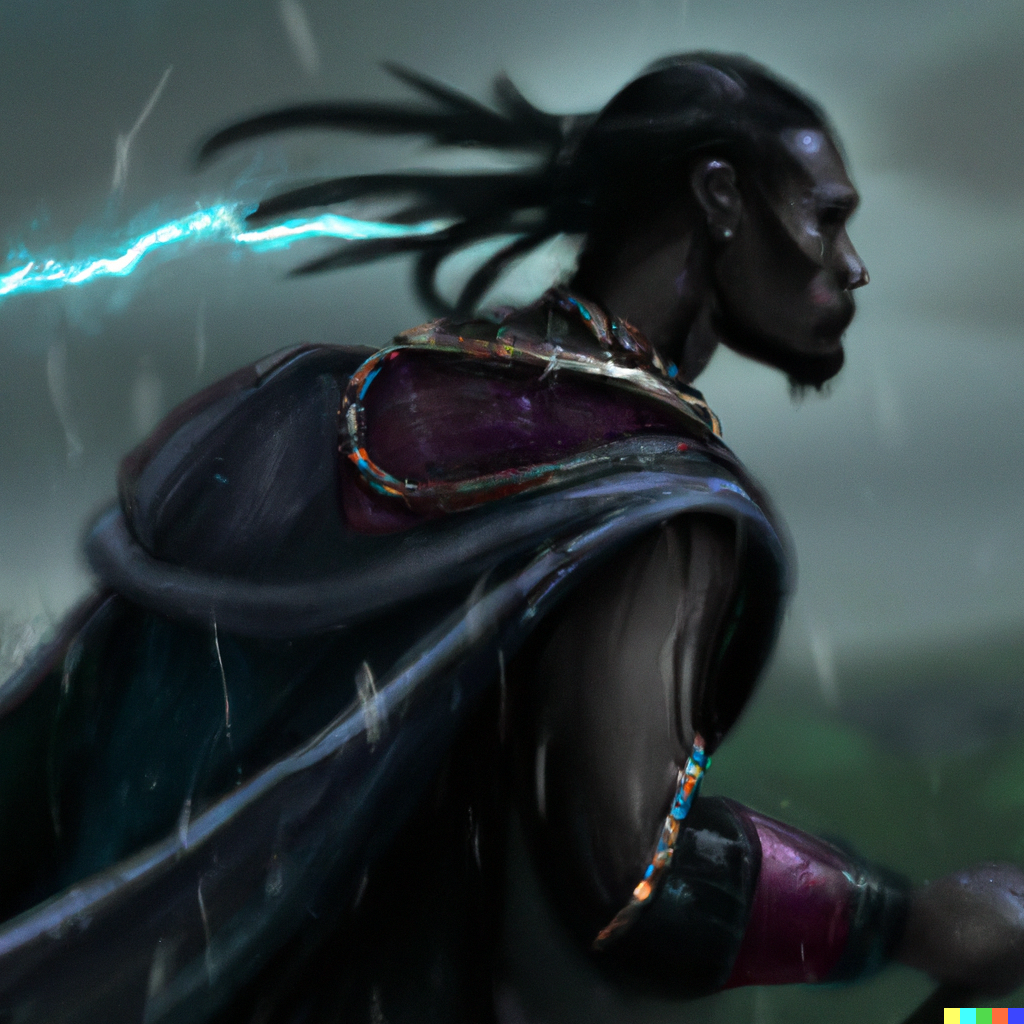
\includegraphics[width=\columnwidth]{equipment/magic apparel}
            Magic apparel items must be worn to gain their effects.

            \subsection{Body Slots}
              The main limiting factor on how many items you can have equipped is your attunement points, not the physical location of your items on your body.
              However, there are limits to how many items you can wear of the same type, as described below.
              For item types not listed here, use reasonable judgment about what would be plausible.
              \begin{itemize}
                \item Amulet: Up to 2
                \item Belt: Up to 2
                \item Boots: Up to 1
                \item Circlet: Up to 2
                \item Cloak: Up to 2
                \item Gauntlets: Up to 1 (separate from gloves)
                \item Gloves: Up to 1 (separate from gauntlets)
                \item Rings: Up to 5 per hand
              \end{itemize}
          \end{longtablepreface}

          
\begin{longtablewrapper}
\begin{longtable}{p{15em} p{3em} p{6em} p{25em} p{3em}}

\lcaption{Apparel Items} \\
\tb{Name} & \tb{Level} & \tb{Typical Price} & \tb{Description} & \tb{Page} \tableheaderrule
Bracers of Archery & \nth{1} & 50 gp & Grants bow proficiency & \pageref{item:Bracers of Archery} \\
Belt of Healing & \nth{2} & 125 gp & Grants healing & \pageref{item:Belt of Healing} \\
Boots of the Winterlands & \nth{2} & 125 gp & Eases travel in cold areas & \pageref{item:Boots of the Winterlands} \\
Bracers of Armor & \nth{2} & 125 gp & Grants invisible armor & \pageref{item:Bracers of Armor} \\
Gauntlets of Improvisation & \nth{2} & 125 gp & Grants \plus1d damage with improvised weapons & \pageref{item:Gauntlets of Improvisation} \\
Ring of Elemental Endurance & \nth{2} & 125 gp & Grants tolerance of temperature extremes & \pageref{item:Ring of Elemental Endurance} \\
Shield of Bashing & \nth{2} & 125 gp & Grants \plus2 power & \pageref{item:Shield of Bashing} \\
Torchlight Gloves & \nth{2} & 125 gp & Sheds light as a torch & \pageref{item:Torchlight Gloves} \\
Ocular Circlet & \nth{3} & 250 gp & Can allow you to see at a distance & \pageref{item:Ocular Circlet} \\
Ring of Nourishment & \nth{3} & 250 gp & Provides food and water & \pageref{item:Ring of Nourishment} \\
Boots of Earth's Embrace & \nth{4} & 500 gp & Grants immunity to forced movement & \pageref{item:Boots of Earth's Embrace} \\
Boots of Elvenkind & \nth{4} & 500 gp & Grants \plus2 Stealth & \pageref{item:Boots of Elvenkind} \\
Circlet of Persuasion & \nth{4} & 500 gp & Grants \plus2 Persuasion & \pageref{item:Circlet of Persuasion} \\
Gauntlet of the Ram & \nth{4} & 500 gp & Knocks back foe when used to strike & \pageref{item:Gauntlet of the Ram} \\
Mask of Water Breathing & \nth{4} & 500 gp & Allows breathing water like air & \pageref{item:Mask of Water Breathing} \\
Throwing Gloves & \nth{4} & 500 gp & Allows throwing any item accurately & \pageref{item:Throwing Gloves} \\
Acid Coated & \nth{5} & 800 gp & Deals acid damage to anything it touches & \pageref{item:Acid Coated} \\
Amulet of Translocation & \nth{5} & 800 gp & Grants ability to teleport up to 30 feet & \pageref{item:Amulet of Translocation} \\
Circlet of Blasting & \nth{5} & 800 gp & Can blast foe with fire & \pageref{item:Circlet of Blasting} \\
Hidden Armor & \nth{5} & 800 gp & Can look like normal clothing & \pageref{item:Hidden Armor} \\
Protective Armor & \nth{5} & 800 gp & Grants \plus1 Armor defense & \pageref{item:Protective Armor} \\
Protective Shield & \nth{5} & 800 gp & Grants \plus1 Armor defense & \pageref{item:Protective Shield} \\
Shield of Arrow Catching & \nth{5} & 800 gp & Redirects small nearby projectiles to hit you & \pageref{item:Shield of Arrow Catching} \\
Shield of Arrow Deflection & \nth{5} & 800 gp & Blocks small projectiles & \pageref{item:Shield of Arrow Deflection} \\
Translocation & \nth{5} & 800 gp & Grants ability to teleport up to 30 feet & \pageref{item:Translocation} \\
Agile & \nth{6} & 1,200 gp & Grants \plus2 Reflex defense & \pageref{item:Agile} \\
Amulet of Health & \nth{6} & 1,200 gp & Grants 2 additional hit points & \pageref{item:Amulet of Health} \\
Amulet of Nondetection & \nth{6} & 1,200 gp & Grants \plus4 to defenses against detection & \pageref{item:Amulet of Nondetection} \\
Boots of Speed & \nth{6} & 1,200 gp & Increases speed by ten feet & \pageref{item:Boots of Speed} \\
Featherlight Armor & \nth{6} & 1,200 gp & Reduces encumbrance by 1 & \pageref{item:Featherlight Armor} \\
Fortified & \nth{6} & 1,200 gp & Grants \plus2 Fortitude defense & \pageref{item:Fortified} \\
Quilled Cloak & \nth{6} & 1,200 gp & Deals damage to creatures that grapple you & \pageref{item:Quilled Cloak} \\
Willguard & \nth{6} & 1,200 gp & Grants \plus2 Mental defense & \pageref{item:Willguard} \\
Anchoring & \nth{7} & 1,800 gp & Protects you from most forced movement attacks & \pageref{item:Anchoring} \\
Armor of Fortification & \nth{7} & 1,800 gp & Reduces critical hits from strikes & \pageref{item:Armor of Fortification} \\
Boots of Water Walking & \nth{7} & 1,800 gp & Allows walking on liquids & \pageref{item:Boots of Water Walking} \\
Boots of the Skydancer & \nth{7} & 1,800 gp & Can walk on air & \pageref{item:Boots of the Skydancer} \\
Bracers of Archery, Greater & \nth{7} & 1,800 gp & Grants bow proficiency, \plus1 ranged accuracy & \pageref{item:Bracers of Archery, Greater} \\
Bracers of Repulsion & \nth{7} & 1,800 gp & Can knock nearby creatures back & \pageref{item:Bracers of Repulsion} \\
Crown of Lightning & \nth{7} & 1,800 gp & Continuously damages nearby enemies & \pageref{item:Crown of Lightning} \\
Gauntlet of the Ram, Greater & \nth{7} & 1,800 gp & Knocks back foe farther when use to strike & \pageref{item:Gauntlet of the Ram, Greater} \\
Gauntlets of Improvisation, Greater & \nth{7} & 1,800 gp & Grants \plus2d damage with improvised weapons & \pageref{item:Gauntlets of Improvisation, Greater} \\
Gloves of Spell Investment & \nth{7} & 1,800 gp & Can invest a spell to cast later & \pageref{item:Gloves of Spell Investment} \\
Hexward Amulet & \nth{7} & 1,800 gp & Grants \plus1 defenses against targeted magical attacks & \pageref{item:Hexward Amulet} \\
Lifekeeping Belt & \nth{7} & 1,800 gp & Grants \plus1 bonus to \glossterm{vital rolls} & \pageref{item:Lifekeeping Belt} \\
Ring of Sustenance & \nth{7} & 1,800 gp & Provides food, water, and rest & \pageref{item:Ring of Sustenance} \\
Amulet of Mighty Fists & \nth{8} & 2,750 gp & Grants \plus2 power with natural and unarmed attacks & \pageref{item:Amulet of Mighty Fists} \\
Armor of Energy Resistance & \nth{8} & 2,750 gp & Reduces energy damage & \pageref{item:Armor of Energy Resistance} \\
Armor of Invulnerability & \nth{8} & 2,750 gp & Reduces physical damage & \pageref{item:Armor of Invulnerability} \\
Assassin's Cloak & \nth{8} & 2,750 gp & Grants invisibility while inactive & \pageref{item:Assassin's Cloak} \\
Avian Cloak & \nth{8} & 2,750 gp & Grants a glide speed & \pageref{item:Avian Cloak} \\
Belt of Healing, Greater & \nth{8} & 2,750 gp & Grants more healing & \pageref{item:Belt of Healing, Greater} \\
Boots of Gravitation & \nth{8} & 2,750 gp & Redirects personal gravity & \pageref{item:Boots of Gravitation} \\
Cloak of Mist & \nth{8} & 2,750 gp & Fills nearby area with fog & \pageref{item:Cloak of Mist} \\
Ring of Protection & \nth{8} & 2,750 gp & Grants \plus1 to Armor and Reflex defenses & \pageref{item:Ring of Protection} \\
Shield of Boulder Catching & \nth{8} & 2,750 gp & Redirects large nearby projectiles to hit you & \pageref{item:Shield of Boulder Catching} \\
Shield of Boulder Deflection & \nth{8} & 2,750 gp & Can block large projectiles & \pageref{item:Shield of Boulder Deflection} \\
Crown of Flame & \nth{9} & 4,000 gp & Grants nearby allies immunity to fire damage & \pageref{item:Crown of Flame} \\
Greatreach Bracers & \nth{9} & 4,000 gp & Increases reach by five feet & \pageref{item:Greatreach Bracers} \\
Hidden Armor, Greater & \nth{9} & 4,000 gp & Can look and sound like normal clothing & \pageref{item:Hidden Armor, Greater} \\
Mask of Air & \nth{9} & 4,000 gp & Allows breathing in any environment & \pageref{item:Mask of Air} \\
Ocular Circlet, Greater & \nth{9} & 4,000 gp & Can allow you to see at a greater distance & \pageref{item:Ocular Circlet, Greater} \\
Ring of Angel's Grace & \nth{9} & 4,000 gp & Grants \plus2 Mental and slows falls & \pageref{item:Ring of Angel's Grace} \\
Boots of Speed, Greater & \nth{10} & 6,500 gp & Increases speed by twenty feet & \pageref{item:Boots of Speed, Greater} \\
Circlet of Blasting, Greater & \nth{10} & 6,500 gp & Can blast foe with intense fire & \pageref{item:Circlet of Blasting, Greater} \\
Crater Boots & \nth{10} & 6,500 gp & Deals your falling damage to enemies & \pageref{item:Crater Boots} \\
Titan Gauntlets & \nth{10} & 6,500 gp & Grants \plus2 \glossterm{mundane} power & \pageref{item:Titan Gauntlets} \\
Winged Boots & \nth{10} & 6,500 gp & Grants limited flight & \pageref{item:Winged Boots} \\
Amulet of Translocation, Greater & \nth{11} & 10,000 gp & Grants ability to teleport up to 100 feet & \pageref{item:Amulet of Translocation, Greater} \\
Crown of Thunder & \nth{11} & 10,000 gp & Continously deafens nearby enemies & \pageref{item:Crown of Thunder} \\
Shield of Arrow Catching, Greater & \nth{11} & 10,000 gp & Selectively redirects small nearby projectiles to hit you & \pageref{item:Shield of Arrow Catching, Greater} \\
Shield of Bashing, Greater & \nth{11} & 10,000 gp & Grants \plus4 power & \pageref{item:Shield of Bashing, Greater} \\
Translocation, Greater & \nth{11} & 10,000 gp & Grants ability to teleport up to 100 feet & \pageref{item:Translocation, Greater} \\
Amulet of the Planes & \nth{12} & 16,000 gp & Aids travel with \ritual{plane shift} & \pageref{item:Amulet of the Planes} \\
Armor of Fortification, Mystic & \nth{12} & 16,000 gp & Reduces critical hits from all attacks & \pageref{item:Armor of Fortification, Mystic} \\
Boots of Freedom & \nth{12} & 16,000 gp & Grants immunity to almost all mobility restrictions & \pageref{item:Boots of Freedom} \\
Featherlight Armor, Greater & \nth{12} & 16,000 gp & Reduces encumbrance by 2 & \pageref{item:Featherlight Armor, Greater} \\
Greater Quilled Cloak & \nth{12} & 16,000 gp & Deals more damage to creatures that grapple you & \pageref{item:Greater Quilled Cloak} \\
Ring of Energy Resistance & \nth{12} & 16,000 gp & Reduces energy damage & \pageref{item:Ring of Energy Resistance} \\
Seven League Boots & \nth{12} & 16,000 gp & Teleport seven leages with a step & \pageref{item:Seven League Boots} \\
Shield of Mystic Reflection & \nth{12} & 16,000 gp & React to reflect magical attacks & \pageref{item:Shield of Mystic Reflection} \\
Anchoring, Greater & \nth{13} & 25,000 gp & Protects you from all forced movement and teleportation attacks & \pageref{item:Anchoring, Greater} \\
Assassin's Cloak, Greater & \nth{13} & 25,000 gp & Grants longer invisibility while inactive & \pageref{item:Assassin's Cloak, Greater} \\
Boots of the Skydancer, Greater & \nth{13} & 25,000 gp & description & \pageref{item:Boots of the Skydancer, Greater} \\
Crown of Frost & \nth{13} & 25,000 gp & Continuously damages nearby enemies & \pageref{item:Crown of Frost} \\
Gloves of Spell Investment, Greater & \nth{13} & 25,000 gp & Can invest two spells to cast later & \pageref{item:Gloves of Spell Investment, Greater} \\
Hexproof Amulet, Greater & \nth{13} & 25,000 gp & Grants \plus2 defenses against targeted magical attacks & \pageref{item:Hexproof Amulet, Greater} \\
Lifekeeping Belt, Greater & \nth{13} & 25,000 gp & Grants \plus2 bonus to \glossterm{vital rolls} & \pageref{item:Lifekeeping Belt, Greater} \\
Vanishing Cloak & \nth{13} & 25,000 gp & Can teleport a short distance and grant invisibility & \pageref{item:Vanishing Cloak} \\
Amulet of Nondetection, Greater & \nth{14} & 37,000 gp & Grants \plus8 to defenses against detection & \pageref{item:Amulet of Nondetection, Greater} \\
Armor of Energy Resistance, Greater & \nth{14} & 37,000 gp & Significantly reduces energy damage & \pageref{item:Armor of Energy Resistance, Greater} \\
Armor of Invulnerability & \nth{14} & 37,000 gp & Significantly reduces physical damage & \pageref{item:Armor of Invulnerability} \\
Belt of Healing, Supreme & \nth{14} & 37,000 gp & Grants more healing & \pageref{item:Belt of Healing, Supreme} \\
Boots of Speed, Supreme & \nth{14} & 37,000 gp & Increases speed by thirty feet & \pageref{item:Boots of Speed, Supreme} \\
Protective Armor, Greater & \nth{14} & 37,000 gp & Grants \plus2 Armor defense & \pageref{item:Protective Armor, Greater} \\
Protective Shield, Greater & \nth{14} & 37,000 gp & Grants \plus2 Armor defense & \pageref{item:Protective Shield, Greater} \\
Shield of Arrow Deflection, Greater & \nth{14} & 37,000 gp & Blocks small projectiles & \pageref{item:Shield of Arrow Deflection, Greater} \\
Agile, Greater & \nth{15} & 55,000 gp & Grants \plus4 Reflex defense & \pageref{item:Agile, Greater} \\
Amulet of Health, Greater & \nth{15} & 55,000 gp & Grants 4 additional hit points & \pageref{item:Amulet of Health, Greater} \\
Armor of Fortification, Greater & \nth{15} & 55,000 gp & Drastically reduces critical hits from strikes & \pageref{item:Armor of Fortification, Greater} \\
Bracers of Repulsion, Greater & \nth{15} & 55,000 gp & Can knock many nearby creatures back & \pageref{item:Bracers of Repulsion, Greater} \\
Fortified, Greater & \nth{15} & 55,000 gp & Grants \plus4 Fortitude defense & \pageref{item:Fortified, Greater} \\
Ring of Regeneration & \nth{15} & 55,000 gp & Automatically removes vital wounds & \pageref{item:Ring of Regeneration} \\
Willguard, Greater & \nth{15} & 55,000 gp & Grants \plus4 Mental defense & \pageref{item:Willguard, Greater} \\
Amulet of Mighty Fists, Greater & \nth{16} & 85,000 gp & Grants \plus4 power with natural and unarmed attacks & \pageref{item:Amulet of Mighty Fists, Greater} \\
Astral Boots & \nth{16} & 85,000 gp & Allows teleporting instead of moving & \pageref{item:Astral Boots} \\
Circlet of Blasting, Supreme & \nth{16} & 85,000 gp & Can blast foe with supremely intense fire & \pageref{item:Circlet of Blasting, Supreme} \\
Cloak of Mist, Greater & \nth{16} & 85,000 gp & Fills nearby area with thick fog & \pageref{item:Cloak of Mist, Greater} \\
Ring of Protection, Greater & \nth{16} & 85,000 gp & Grants \plus2 to Armor and Reflex defenses & \pageref{item:Ring of Protection, Greater} \\
Amulet of Translocation, Supreme & \nth{17} & 125,000 gp & Grants ability to teleport up to 300 feet & \pageref{item:Amulet of Translocation, Supreme} \\
Greatreach Bracers, Greater & \nth{17} & 125,000 gp & Increases reach by ten feet & \pageref{item:Greatreach Bracers, Greater} \\
Shield of Boulder Deflection, Greater & \nth{17} & 125,000 gp & Blocks large projectiles & \pageref{item:Shield of Boulder Deflection, Greater} \\
Translocation, Supreme & \nth{17} & 125,000 gp & Grants ability to teleport up to 300 feet & \pageref{item:Translocation, Supreme} \\
Featherlight Armor, Supreme & \nth{18} & 190,000 gp & Reduces encumbrance by 2 & \pageref{item:Featherlight Armor, Supreme} \\
Supreme Quilled Cloak & \nth{18} & 190,000 gp & Deals even more damage to creatures that grapple you & \pageref{item:Supreme Quilled Cloak} \\
Hexproof Amulet, Supreme & \nth{19} & 280,000 gp & Grants \plus3 defenses against targeted magical attacks & \pageref{item:Hexproof Amulet, Supreme} \\
Lifekeeping Belt, Supreme & \nth{19} & 280,000 gp & Grants \plus3 bonus to \glossterm{vital rolls} & \pageref{item:Lifekeeping Belt, Supreme} \\
Titan Gauntlets, Greater & \nth{19} & 280,000 gp & Grants \plus4 \glossterm{mundane} power & \pageref{item:Titan Gauntlets, Greater} \\
Armor of Energy Resistance, Supreme & \nth{20} & 400,000 gp & Drastically reduces energy damage & \pageref{item:Armor of Energy Resistance, Supreme} \\
Armor of Invulnerability, Greater & \nth{20} & 400,000 gp & Drastically reduces physical damage & \pageref{item:Armor of Invulnerability, Greater} \\
Shield of Bashing, Supreme & \nth{20} & 400,000 gp & Grants \plus6 power & \pageref{item:Shield of Bashing, Supreme} \\

\end{longtable}
\end{longtablewrapper}


      \end{longcolumn}
\section{Magic Apparel Descriptions}

  \lowercase{\hypertarget{item:Amulet of Mighty Fists}{}}\label{item:Amulet of Mighty Fists}
\hypertarget{item:Amulet of Mighty Fists}{\subsubsection{Amulet of Mighty Fists\hfill\nth{6}}}
You gain a \plus1d bonus to \glossterm{strike damage} with \glossterm{unarmed attacks} and natural weapons.
\parhead*{Tags} \glossterm{Enhancement}
\parhead*{Materials} Jewelry
\lowercase{\hypertarget{item:Amulet of Mighty Fists, Greater}{}}\label{item:Amulet of Mighty Fists, Greater}
\hypertarget{item:Amulet of Mighty Fists, Greater}{\subsubsection{Amulet of Mighty Fists, Greater\hfill\nth{14}}}
You gain a \plus2d bonus to \glossterm{strike damage} with \glossterm{unarmed attacks} and natural weapons.
\parhead*{Tags} \glossterm{Enhancement}
\parhead*{Materials} Jewelry
\lowercase{\hypertarget{item:Armor of Energy Resistance}{}}\label{item:Armor of Energy Resistance}
\hypertarget{item:Armor of Energy Resistance}{\subsubsection{Armor of Energy Resistance\hfill\nth{4}}}
You have \glossterm{damage reduction} equal to the item's \glossterm{power} against \glossterm{energy damage}.
Whenever you resist energy with this item, it sheds light as a torch until the end of the next round.
The color of the light depends on the energy damage resisted: blue for cold, yellow for electricity, red for fire, and brown for sonic.
\parhead*{Tags} \glossterm{Shielding}
\parhead*{Materials} Bone, metal
\lowercase{\hypertarget{item:Armor of Energy Resistance, Greater}{}}\label{item:Armor of Energy Resistance, Greater}
\hypertarget{item:Armor of Energy Resistance, Greater}{\subsubsection{Armor of Energy Resistance, Greater\hfill\nth{12}}}
This item functions like the \mitem{armor of energy resistance} item, except that the damage reduction is equal to twice the item's \glossterm{power}.
\parhead*{Tags} \glossterm{Shielding}
\parhead*{Materials} Bone, metal
\lowercase{\hypertarget{item:Armor of Fortification}{}}\label{item:Armor of Fortification}
\hypertarget{item:Armor of Fortification}{\subsubsection{Armor of Fortification\hfill\nth{7}}}
You gain a \plus5 bonus to defenses when determining whether a \glossterm{strike} gets a \glossterm{critical hit} against you instead of a normal hit.
\parhead*{Tags} \glossterm{Imbuement}
\parhead*{Materials} Bone, metal
\lowercase{\hypertarget{item:Armor of Fortification, Greater}{}}\label{item:Armor of Fortification, Greater}
\hypertarget{item:Armor of Fortification, Greater}{\subsubsection{Armor of Fortification, Greater\hfill\nth{15}}}
This item functions like the \mitem{armor of fortification} item, except that the bonus increases to \plus10.
\parhead*{Tags} \glossterm{Imbuement}
\parhead*{Materials} Bone, metal
\lowercase{\hypertarget{item:Armor of Fortification, Mystic}{}}\label{item:Armor of Fortification, Mystic}
\hypertarget{item:Armor of Fortification, Mystic}{\subsubsection{Armor of Fortification, Mystic\hfill\nth{12}}}
This item functions like the \mitem{armor of fortification} item, except that it applies against all attacks instead of only against; \glossterm{strikes}.
\parhead*{Tags} \glossterm{Imbuement}
\parhead*{Materials} Bone, metal
\lowercase{\hypertarget{item:Armor of Invulnerability}{}}\label{item:Armor of Invulnerability}
\hypertarget{item:Armor of Invulnerability}{\subsubsection{Armor of Invulnerability\hfill\nth{8}}}
You have \glossterm{damage reduction} equal to this item's \glossterm{power} against damage from \glossterm{physical attacks}.
\parhead*{Tags} \glossterm{Shielding}
\parhead*{Materials} Bone, metal
\lowercase{\hypertarget{item:Armor of Invulnerability, Greater}{}}\label{item:Armor of Invulnerability, Greater}
\hypertarget{item:Armor of Invulnerability, Greater}{\subsubsection{Armor of Invulnerability, Greater\hfill\nth{16}}}
This item functions like the \mitem{armor of invulnerability} item, except that the damage reduction is equal to twice the item's \glossterm{power}.
You have \glossterm{damage reduction} equal to the item's \glossterm{power} against damage from \glossterm{physical attacks}.
\parhead*{Tags} \glossterm{Shielding}
\parhead*{Materials} Bone, metal
\lowercase{\hypertarget{item:Armor of Magic Resistance}{}}\label{item:Armor of Magic Resistance}
\hypertarget{item:Armor of Magic Resistance}{\subsubsection{Armor of Magic Resistance\hfill\nth{14}}}
You have \glossterm{magic resistance} equal to 5 + the item's \glossterm{power}.
\parhead*{Tags} \glossterm{Shielding}
\parhead*{Materials} Bone, metal
\lowercase{\hypertarget{item:Assassin's Cloak}{}}\label{item:Assassin's Cloak}
\hypertarget{item:Assassin's Cloak}{\subsubsection{Assassin's Cloak\hfill\nth{7}}}
At the end of each round, if you took no actions that round, you become \glossterm{invisible} until the end of the next round.
\parhead*{Tags} \glossterm{Glamer}
\parhead*{Materials} Textiles
\lowercase{\hypertarget{item:Assassin's Cloak, Greater}{}}\label{item:Assassin's Cloak, Greater}
\hypertarget{item:Assassin's Cloak, Greater}{\subsubsection{Assassin's Cloak, Greater\hfill\nth{17}}}
At the end of each round, if you did not attack a creature that round, you become \glossterm{invisible} until the end of the next round.
\parhead*{Tags} \glossterm{Glamer}
\parhead*{Materials} Textiles
\lowercase{\hypertarget{item:Astral Boots}{}}\label{item:Astral Boots}
\hypertarget{item:Astral Boots}{\subsubsection{Astral Boots\hfill\nth{16}}}
Whenever you move, you can teleport the same distance instead.
This does not change the total distance you can move, but you can teleport in any direction, even vertically.
You cannot teleport to locations you do not have \glossterm{line of sight} and \glossterm{line of effect} to.
\parhead*{Tags} \glossterm{Teleportation}
\parhead*{Materials} Bone, leather, metal
\lowercase{\hypertarget{item:Belt of Healing}{}}\label{item:Belt of Healing}
\hypertarget{item:Belt of Healing}{\subsubsection{Belt of Healing\hfill\nth{1}}}
When you use the \textit{recover} action, you heal \plus1d hit points.
\parhead*{Tags} \glossterm{Life}
\parhead*{Materials} Leather, textiles
\lowercase{\hypertarget{item:Belt of Healing, Greater}{}}\label{item:Belt of Healing, Greater}
\hypertarget{item:Belt of Healing, Greater}{\subsubsection{Belt of Healing, Greater\hfill\nth{8}}}
When you use the \textit{recover} action, you heal \plus2d hit points.
\parhead*{Tags} \glossterm{Life}
\parhead*{Materials} Leather, textiles
\lowercase{\hypertarget{item:Belt of Heroic Recovery}{}}\label{item:Belt of Heroic Recovery}
\hypertarget{item:Belt of Heroic Recovery}{\subsubsection{Belt of Heroic Recovery\hfill\nth{6}}}
% TODO: timing?
As an \glossterm{immediate action} when you get a \glossterm{critical hit}, you can take the \textit{recover} action.
\parhead*{Tags} \glossterm{Life}
\parhead*{Materials} Leather, textiles
\lowercase{\hypertarget{item:Boots of Earth's Embrace}{}}\label{item:Boots of Earth's Embrace}
\hypertarget{item:Boots of Earth's Embrace}{\subsubsection{Boots of Earth's Embrace\hfill\nth{4}}}
While you are standing on solid ground, you are immune to effects that would force you to move.
This does not protect you from other effects of those attacks, such as damage.
\parhead*{Tags} \glossterm{Earth}, \glossterm{Enhancement}
\parhead*{Materials} Bone, leather, metal
\lowercase{\hypertarget{item:Boots of Freedom}{}}\label{item:Boots of Freedom}
\hypertarget{item:Boots of Freedom}{\subsubsection{Boots of Freedom\hfill\nth{6}}}
You are immune to effects that restrict your mobility.
This removes all penalties you would suffer for acting underwater, except for those relating to using ranged weapons.
This does not prevent you from being \grappled, but you gain a \plus10 bonus to your defense against \glossterm{grapple} attacks.
\parhead*{Tags} \glossterm{Imbuement}
\parhead*{Materials} Bone, leather, metal
\lowercase{\hypertarget{item:Boots of Freedom, Greater}{}}\label{item:Boots of Freedom, Greater}
\hypertarget{item:Boots of Freedom, Greater}{\subsubsection{Boots of Freedom, Greater\hfill\nth{12}}}
These boots function like \mitem{boots of freedom}, except that you are also immune to being \grappled.
\parhead*{Tags} \glossterm{Imbuement}
\parhead*{Materials} Bone, leather, metal
\lowercase{\hypertarget{item:Boots of Gravitation}{}}\label{item:Boots of Gravitation}
\hypertarget{item:Boots of Gravitation}{\subsubsection{Boots of Gravitation\hfill\nth{8}}}
While these boots are within 5 feet of a solid surface, gravity pulls you towards the solid surface closest to your boots rather than in the normal direction.
This can allow you to walk easily on walls or even ceilings.
\parhead*{Tags} \glossterm{Imbuement}
\parhead*{Materials} Bone, leather, metal
\lowercase{\hypertarget{item:Boots of Speed}{}}\label{item:Boots of Speed}
\hypertarget{item:Boots of Speed}{\subsubsection{Boots of Speed\hfill\nth{5}}}
You gain a \plus10 foot bonus to your speed in all your movement modes, up to a maximum of double your normal speed.
\parhead*{Tags} \glossterm{Temporal}
\parhead*{Materials} Bone, leather, metal
\lowercase{\hypertarget{item:Boots of Speed, Greater}{}}\label{item:Boots of Speed, Greater}
\hypertarget{item:Boots of Speed, Greater}{\subsubsection{Boots of Speed, Greater\hfill\nth{13}}}
You gain a \plus30 foot bonus to your speed in all your movement modes, up to a maximum of double your normal speed.
\parhead*{Tags} \glossterm{Temporal}
\parhead*{Materials} Bone, leather, metal
\lowercase{\hypertarget{item:Boots of Water Walking}{}}\label{item:Boots of Water Walking}
\hypertarget{item:Boots of Water Walking}{\subsubsection{Boots of Water Walking\hfill\nth{7}}}
You treat the surface of all liquids as if they were firm ground.
Your feet hover about an inch above the liquid's surface, allowing you to traverse dangerous liquids without harm as long as the surface is calm.
If you are below the surface of the liquid, you rise towards the surface at a rate of 60 feet per round.
Thick liquids, such as mud and lava, may cause you to rise more slowly.
\parhead*{Tags} \glossterm{Imbuement}
\parhead*{Materials} Bone, leather, metal
\lowercase{\hypertarget{item:Boots of the Winterlands}{}}\label{item:Boots of the Winterlands}
\hypertarget{item:Boots of the Winterlands}{\subsubsection{Boots of the Winterlands\hfill\nth{2}}}
You can travel across snow and ice without slipping or suffering movement penalties for the terrain.
% TODO: degree symbol?
In addition, the boots keep you warn, protecting you in environments as cold as \minus50 Fahrenheit.
\parhead*{Tags} \glossterm{Enhancement}
\parhead*{Materials} Bone, leather, metal
\lowercase{\hypertarget{item:Bracers of Archery}{}}\label{item:Bracers of Archery}
\hypertarget{item:Bracers of Archery}{\subsubsection{Bracers of Archery\hfill\nth{1}}}
You are proficient with bows.
\parhead*{Tags} \glossterm{Enhancement}
\parhead*{Materials} Bone, leather, metal, wood
\lowercase{\hypertarget{item:Bracers of Armor}{}}\label{item:Bracers of Armor}
\hypertarget{item:Bracers of Armor}{\subsubsection{Bracers of Armor\hfill\nth{2}}}
You gain a \plus2 bonus to Armor defense.
The protection from these bracers is treated as body armor, and it does not stack with any other body armor you wear.
\parhead*{Tags} \glossterm{Shielding}
\parhead*{Materials} Bone, leather, metal, wood
\lowercase{\hypertarget{item:Bracers of Repulsion}{}}\label{item:Bracers of Repulsion}
\hypertarget{item:Bracers of Repulsion}{\subsubsection{Bracers of Repulsion\hfill\nth{4}}}
Whenever a creature hits you with a melee \glossterm{strike} during the \glossterm{action phase},
you can spend an \glossterm{action point} to use this item as an \glossterm{immediate action}.
If you do, you make a \glossterm{shove} attack against that creature during the \glossterm{delayed action phase}, using this item's power in place of your Strength.
\parhead*{Tags} \glossterm{Telekinesis}
\parhead*{Materials} Bone, leather, metal, wood
\lowercase{\hypertarget{item:Bracers of Repulsion, Greater}{}}\label{item:Bracers of Repulsion, Greater}
\hypertarget{item:Bracers of Repulsion, Greater}{\subsubsection{Bracers of Repulsion, Greater\hfill\nth{11}}}
This item functions like the \mitem{bracers of repulsion} item, except that it does not cost an action point to use.
\parhead*{Tags} \glossterm{Telekinesis}
\parhead*{Materials} Bone, leather, metal, wood
\lowercase{\hypertarget{item:Cloak of Mist}{}}\label{item:Cloak of Mist}
\hypertarget{item:Cloak of Mist}{\subsubsection{Cloak of Mist\hfill\nth{8}}}
Fog constantly fills an \areamed radius emanation from you.
This fog does not fully block sight, but it provides \concealment.
If a 5-foot square of fog takes fire damage equal to half this item's \glossterm{power}, the fog disappears from that area until the end of the next round.
\parhead*{Tags} \glossterm{Fog}, \glossterm{Manifestation}
\parhead*{Materials} Textiles
\lowercase{\hypertarget{item:Cloak of Mist, Greater}{}}\label{item:Cloak of Mist, Greater}
\hypertarget{item:Cloak of Mist, Greater}{\subsubsection{Cloak of Mist, Greater\hfill\nth{16}}}
A thick fog constantly fills an \areamed radius emanation from you.
This fog completely blocks sight beyond 10 feet.
Within that range, it still provides \concealment.
If a 5-foot square of fog takes fire damage equal to this item's \glossterm{power}, the fog disappears from that area until the end of the next round.
\parhead*{Tags} \glossterm{Fog}, \glossterm{Manifestation}
\parhead*{Materials} Textiles
\lowercase{\hypertarget{item:Crown of Flame}{}}\label{item:Crown of Flame}
\hypertarget{item:Crown of Flame}{\subsubsection{Crown of Flame\hfill\nth{5}}}
This crown is continuously on fire.
The flame sheds light as a torch.
You and all allies within an \arealarge radius emanation from you are immune to fire damage.
\parhead*{Tags} \glossterm{Fire}
\parhead*{Materials} Bone, metal
\lowercase{\hypertarget{item:Crown of Frost}{}}\label{item:Crown of Frost}
\hypertarget{item:Crown of Frost}{\subsubsection{Crown of Frost\hfill\nth{11}}}
At the end of each \glossterm{action phase}, you make a Power vs. Fortitude attack against all enemies within an \areamed radius emanation from you.
A hit deals cold \glossterm{standard damage} \minus3d.
Each creature that takes damage in this way is \fatigued until the end of the next round.
\parhead*{Tags} \glossterm{Cold}
\parhead*{Materials} Bone, metal
\lowercase{\hypertarget{item:Crown of Lightning}{}}\label{item:Crown of Lightning}
\hypertarget{item:Crown of Lightning}{\subsubsection{Crown of Lightning\hfill\nth{7}}}
This crown continuously crackles with electricity.
The constant sparks shed light as a torch.
At the end of each \glossterm{action phase}, you make a Power vs. Reflex attack against all enemies within an \areamed radius emanation from you.
A hit deals electricity \glossterm{standard damage} \minus3d.
\parhead*{Tags} \glossterm{Electricity}
\parhead*{Materials} Bone, metal
\lowercase{\hypertarget{item:Crown of Thunder}{}}\label{item:Crown of Thunder}
\hypertarget{item:Crown of Thunder}{\subsubsection{Crown of Thunder\hfill\nth{9}}}
The crown constantly emits a low-pitched rumbling.
To you and your allies, the sound is barely perceptible.
However, all enemies within an \arealarge radius emanation from you hear the sound as a deafening, continuous roll of thunder.
The noise blocks out all other sounds quieter than thunder, causing them to be \deafened while they remain in the area and until the end of the next round after they leave.
\parhead*{Tags} \glossterm{Sonic}
\parhead*{Materials} Bone, metal
\lowercase{\hypertarget{item:Featherlight Armor}{}}\label{item:Featherlight Armor}
\hypertarget{item:Featherlight Armor}{\subsubsection{Featherlight Armor\hfill\nth{4}}}
This armor's \glossterm{encumbrance penalty} is reduced by 2.
\parhead*{Tags} \glossterm{Enhancement}
\parhead*{Materials} Bone, metal
\lowercase{\hypertarget{item:Featherlight Armor, Greater}{}}\label{item:Featherlight Armor, Greater}
\hypertarget{item:Featherlight Armor, Greater}{\subsubsection{Featherlight Armor, Greater\hfill\nth{10}}}
This armor's \glossterm{encumbrance penalty} is reduced by 4.
\parhead*{Tags} \glossterm{Enhancement}
\parhead*{Materials} Bone, metal
\lowercase{\hypertarget{item:Gauntlet of the Ram}{}}\label{item:Gauntlet of the Ram}
\hypertarget{item:Gauntlet of the Ram}{\subsubsection{Gauntlet of the Ram\hfill\nth{2}}}
If you hit on a \glossterm{strike} with this gauntlet during the \glossterm{action phse}, you can attempt to \glossterm{shove} your foe during the \glossterm{delayed action phase}.
Making a strike with this gauntlet is equivalent to an \glossterm{unarmed attack}.
You do not need to move with your foe to push it back the full distance.
\parhead*{Tags} \glossterm{Telekinesis}
\parhead*{Materials} Bone, metal, wood
\lowercase{\hypertarget{item:Gauntlet of the Ram, Greater}{}}\label{item:Gauntlet of the Ram, Greater}
\hypertarget{item:Gauntlet of the Ram, Greater}{\subsubsection{Gauntlet of the Ram, Greater\hfill\nth{7}}}
This item functions like the \mitem{gauntlet of the ram}, except that you gain a bonus to the \glossterm{shove} attack equal to the damage you dealt with the \glossterm{strike}.
\parhead*{Tags} \glossterm{Telekinesis}
\parhead*{Materials} Bone, metal, wood
\lowercase{\hypertarget{item:Gauntlets of Improvisation}{}}\label{item:Gauntlets of Improvisation}
\hypertarget{item:Gauntlets of Improvisation}{\subsubsection{Gauntlets of Improvisation\hfill\nth{2}}}
You gain a \plus1d bonus to damage with \glossterm{improvised weapons}.
\parhead*{Tags} \glossterm{Enhancement}
\parhead*{Materials} Bone, metal, wood
\lowercase{\hypertarget{item:Gauntlets of Improvisation, Greater}{}}\label{item:Gauntlets of Improvisation, Greater}
\hypertarget{item:Gauntlets of Improvisation, Greater}{\subsubsection{Gauntlets of Improvisation, Greater\hfill\nth{7}}}
This item functions like the \mitem{gauntlets of improvisation}, except that the damage bonus is increased to \plus2d.
\parhead*{Tags} \glossterm{Enhancement}
\parhead*{Materials} Bone, metal, wood
\lowercase{\hypertarget{item:Greatreach Bracers}{}}\label{item:Greatreach Bracers}
\hypertarget{item:Greatreach Bracers}{\subsubsection{Greatreach Bracers\hfill\nth{9}}}
Your \glossterm{reach} is increased by 5 feet.
\parhead*{Tags} \glossterm{Imbuement}
\parhead*{Materials} Bone, leather, metal, wood
\lowercase{\hypertarget{item:Greatreach Bracers, Greater}{}}\label{item:Greatreach Bracers, Greater}
\hypertarget{item:Greatreach Bracers, Greater}{\subsubsection{Greatreach Bracers, Greater\hfill\nth{17}}}
Your \glossterm{reach} is increased by 10 feet.
\parhead*{Tags} \glossterm{Imbuement}
\parhead*{Materials} Bone, leather, metal, wood
\lowercase{\hypertarget{item:Hexproof Cloak}{}}\label{item:Hexproof Cloak}
\hypertarget{item:Hexproof Cloak}{\subsubsection{Hexproof Cloak\hfill\nth{18}}}
All \glossterm{magical} abilities that target you directly fail to affect you.
This does not protect you from abilities that affect an area.
\parhead*{Tags} \glossterm{Thaumaturgy}
\parhead*{Materials} Textiles
\lowercase{\hypertarget{item:Hexward Cloak}{}}\label{item:Hexward Cloak}
\hypertarget{item:Hexward Cloak}{\subsubsection{Hexward Cloak\hfill\nth{10}}}
You gain a \plus5 bonus to defenses against \glossterm{magical} abilities that target you directly.
This does not protect you from abilities that affect an area.
\parhead*{Tags} \glossterm{Thaumaturgy}
\parhead*{Materials} Textiles
\lowercase{\hypertarget{item:Hidden Armor}{}}\label{item:Hidden Armor}
\hypertarget{item:Hidden Armor}{\subsubsection{Hidden Armor\hfill\nth{4}}}
As a standard action, you can use this item.
If you do, it appears to change shape and form to assume the shape of a normal set of clothing.
You may choose the design of the clothing.
The item retains all of its properties, including weight and sound, while disguised in this way.
Only its visual appearance is altered.
Alternately, you may return the armor to its original appearance.
\parhead*{Tags} \glossterm{Glamer}
\parhead*{Materials} Bone, metal
\lowercase{\hypertarget{item:Hidden Armor, Greater}{}}\label{item:Hidden Armor, Greater}
\hypertarget{item:Hidden Armor, Greater}{\subsubsection{Hidden Armor, Greater\hfill\nth{9}}}
This item functions like the \mitem{hidden armor} item, except that the item also makes sound appropriate to its disguised form while disguised.
\parhead*{Tags} \glossterm{Alteration}
\parhead*{Materials} Bone, metal
\lowercase{\hypertarget{item:Mask of Air}{}}\label{item:Mask of Air}
\hypertarget{item:Mask of Air}{\subsubsection{Mask of Air\hfill\nth{9}}}
If you breathe through this mask, you breathe in clean, fresh air, regardless of your environment.
This can protect you from inhaled poisons and similar effects.
\parhead*{Tags} \glossterm{Imbuement}
\parhead*{Materials} Textiles
\lowercase{\hypertarget{item:Mask of Water Breathing}{}}\label{item:Mask of Water Breathing}
\hypertarget{item:Mask of Water Breathing}{\subsubsection{Mask of Water Breathing\hfill\nth{4}}}
You can breathe water through this mask as easily as a human breaths air.
This does not grant you the ability to breathe other liquids.
\parhead*{Tags} \glossterm{Imbuement}
\parhead*{Materials} Textiles
\lowercase{\hypertarget{item:Ring of Elemental Endurance}{}}\label{item:Ring of Elemental Endurance}
\hypertarget{item:Ring of Elemental Endurance}{\subsubsection{Ring of Elemental Endurance\hfill\nth{2}}}
You can exist comfortably in conditions between \minus50 and 140 degrees Fahrenheit without any ill effects.
You suffer the normal penalties in temperatures outside of that range.
\parhead*{Tags} \glossterm{Shielding}
\parhead*{Materials} Bone, jewelry, metal, wood
\lowercase{\hypertarget{item:Ring of Energy Resistance}{}}\label{item:Ring of Energy Resistance}
\hypertarget{item:Ring of Energy Resistance}{\subsubsection{Ring of Energy Resistance\hfill\nth{6}}}
You have \glossterm{damage reduction} equal to the ring's \glossterm{power} against \glossterm{energy damage}.
Whenever you resist energy with this ability, the ring sheds light as a torch until the end of the next round.
The color of the light depends on the energy damage resisted: blue for cold, yellow for electricity, red for fire, and brown for sonic.
\parhead*{Tags} \glossterm{Shielding}
\parhead*{Materials} Bone, jewelry, metal, wood
\lowercase{\hypertarget{item:Ring of Energy Resistance, Greater}{}}\label{item:Ring of Energy Resistance, Greater}
\hypertarget{item:Ring of Energy Resistance, Greater}{\subsubsection{Ring of Energy Resistance, Greater\hfill\nth{14}}}
This item functions like the \mitem{ring of energy resistance}, except that the damage reduction is equal to twice the item's \glossterm{power}.
\parhead*{Tags} \glossterm{Shielding}
\parhead*{Materials} Bone, jewelry, metal, wood
\lowercase{\hypertarget{item:Ring of Nourishment}{}}\label{item:Ring of Nourishment}
\hypertarget{item:Ring of Nourishment}{\subsubsection{Ring of Nourishment\hfill\nth{3}}}
You continuously gain nourishment, and no longer need to eat or drink.
This ring must be worn for 24 hours before it begins to work.
\parhead*{Tags} \glossterm{Creation}
\parhead*{Materials} Bone, jewelry, metal, wood
\lowercase{\hypertarget{item:Ring of Protection}{}}\label{item:Ring of Protection}
\hypertarget{item:Ring of Protection}{\subsubsection{Ring of Protection\hfill\nth{8}}}
You gain a \plus1 bonus to Armor defense.
\parhead*{Tags} \glossterm{Shielding}
\parhead*{Materials} Bone, jewelry, metal, wood
\lowercase{\hypertarget{item:Ring of Regeneration}{}}\label{item:Ring of Regeneration}
\hypertarget{item:Ring of Regeneration}{\subsubsection{Ring of Regeneration\hfill\nth{11}}}
At the end of each \glossterm{action phase}, you heal hit points equal to this item's \glossterm{power}.
Only damage taken while wearing the ring can be healed in this way.
\parhead*{Tags} \glossterm{Life}
\parhead*{Materials} Bone, jewelry, metal, wood
\lowercase{\hypertarget{item:Ring of Sustenance}{}}\label{item:Ring of Sustenance}
\hypertarget{item:Ring of Sustenance}{\subsubsection{Ring of Sustenance\hfill\nth{7}}}
You continuously gain nourishment, and no longer need to eat or drink.
In addition, you need only one-quarter your normal amount of sleep (or similar activity, such as elven trance) each day.
The ring must be worn for 24 hours before it begins to work.
\parhead*{Tags} \glossterm{Creation}, \glossterm{Temporal}
\parhead*{Materials} Bone, jewelry, metal, wood
\lowercase{\hypertarget{item:Seven League Boots}{}}\label{item:Seven League Boots}
\hypertarget{item:Seven League Boots}{\subsubsection{Seven League Boots\hfill\nth{12}}}
As a standard action, you can spend an \glossterm{action point} to use this item.
If you do, you teleport exactly 25 miles in a direction you specify.
If this would place you within a solid object or otherwise impossible space, the boots will shunt you up to 1,000 feet in any direction to the closest available space.
If there is no available space within 1,000 feet of your intended destination, the effect fails and you take \glossterm{standard damage} \minus1d.
\parhead*{Tags} \glossterm{Teleportation}
\parhead*{Materials} Bone, leather, metal
\lowercase{\hypertarget{item:Shield of Arrow Catching}{}}\label{item:Shield of Arrow Catching}
\hypertarget{item:Shield of Arrow Catching}{\subsubsection{Shield of Arrow Catching\hfill\nth{5}}}
Whenever a creature within a \areamed radius emanation from you would be attacked by a ranged weapon, the attack is redirected to target you instead.
Resolve the attack as if it had initially targeted you, except that the attack is not affected by cover or concealment.
This item can only affect projectiles and thrown objects that are Small or smaller.
\parhead*{Tags} \glossterm{Telekinesis}
\parhead*{Materials} Bone, metal, wood
\lowercase{\hypertarget{item:Shield of Arrow Catching, Greater}{}}\label{item:Shield of Arrow Catching, Greater}
\hypertarget{item:Shield of Arrow Catching, Greater}{\subsubsection{Shield of Arrow Catching, Greater\hfill\nth{10}}}
This item functions like the \mitem{shield of arrow catching} item, except that it affects a \arealarge radius from you.
In addition, you may choose to exclude creature from this item's effect, allowing projectiles to target nearby foes normally.
\parhead*{Tags} \glossterm{Telekinesis}
\parhead*{Materials} Bone, metal, wood
\lowercase{\hypertarget{item:Shield of Arrow Deflection}{}}\label{item:Shield of Arrow Deflection}
\hypertarget{item:Shield of Arrow Deflection}{\subsubsection{Shield of Arrow Deflection\hfill\nth{2}}}
As an \glossterm{immediate action} when you are attacked by a ranged \glossterm{strike}, you can use this item.
If you do, you gain a \plus5 bonus to Armor defense against the attack.
You must be aware of the attack to deflect it in this way.
This item can only affect projectiles and thrown objects that are Small or smaller.
\parhead*{Tags} \glossterm{Telekinesis}
\parhead*{Materials} Bone, metal, wood
\lowercase{\hypertarget{item:Shield of Arrow Deflection, Greater}{}}\label{item:Shield of Arrow Deflection, Greater}
\hypertarget{item:Shield of Arrow Deflection, Greater}{\subsubsection{Shield of Arrow Deflection, Greater\hfill\nth{12}}}
This item functions like the \mitem{shield of arrow deflection} item, except that the defense bonus increases to \plus10.
\parhead*{Tags} \glossterm{Telekinesis}
\parhead*{Materials} Bone, metal, wood
\lowercase{\hypertarget{item:Shield of Bashing}{}}\label{item:Shield of Bashing}
\hypertarget{item:Shield of Bashing}{\subsubsection{Shield of Bashing\hfill\nth{2}}}
% Should this be strike damage?
You gain a \plus1d bonus to damage with \glossterm{physical attacks} using this shield.
\parhead*{Tags} \glossterm{Enhancement}
\parhead*{Materials} Bone, metal, wood
\lowercase{\hypertarget{item:Shield of Bashing, Greater}{}}\label{item:Shield of Bashing, Greater}
\hypertarget{item:Shield of Bashing, Greater}{\subsubsection{Shield of Bashing, Greater\hfill\nth{11}}}
% Should this be strike damage?
You gain a \plus2d bonus to damage with \glossterm{physical attacks} using this shield.
\parhead*{Tags} \glossterm{Enhancement}
\parhead*{Materials} Bone, metal, wood
\lowercase{\hypertarget{item:Shield of Boulder Catching}{}}\label{item:Shield of Boulder Catching}
\hypertarget{item:Shield of Boulder Catching}{\subsubsection{Shield of Boulder Catching\hfill\nth{8}}}
This item functions like the \mitem{shield of arrow catching} item, except that it can affect projectile and thrown objects of up to Large size.
\parhead*{Tags} \glossterm{Telekinesis}
\parhead*{Materials} Bone, metal, wood
\lowercase{\hypertarget{item:Shield of Boulder Deflection}{}}\label{item:Shield of Boulder Deflection}
\hypertarget{item:Shield of Boulder Deflection}{\subsubsection{Shield of Boulder Deflection\hfill\nth{6}}}
This item functions like the \mitem{shield of arrow deflection} item, except that it can affect projectiles and thrown objects of up to Large size.
\parhead*{Tags} \glossterm{Telekinesis}
\parhead*{Materials} Bone, metal, wood
\lowercase{\hypertarget{item:Shield of Mystic Reflection}{}}\label{item:Shield of Mystic Reflection}
\hypertarget{item:Shield of Mystic Reflection}{\subsubsection{Shield of Mystic Reflection\hfill\nth{12}}}
As an \glossterm{immediate action} when you are targeted by a targeted \glossterm{magical} ability, you can spend an \glossterm{action point} to use this ability.
If you do, the ability targets the creature using the ability instead of you.
Any other targets of the ability are affected normally.
\parhead*{Tags} \glossterm{Thaumaturgy}
\parhead*{Materials} Bone, metal, wood
\lowercase{\hypertarget{item:Throwing Gloves}{}}\label{item:Throwing Gloves}
\hypertarget{item:Throwing Gloves}{\subsubsection{Throwing Gloves\hfill\nth{4}}}
% TODO: reference basic "not designed to be thrown" mechanics?
You can throw any item as if it was designed to be thrown.
This does not improve your ability to throw items designed to be thrown, such as darts.
\parhead*{Tags} \glossterm{Enhancement}
\parhead*{Materials} Leather
\lowercase{\hypertarget{item:Torchlight Gloves}{}}\label{item:Torchlight Gloves}
\hypertarget{item:Torchlight Gloves}{\subsubsection{Torchlight Gloves\hfill\nth{2}}}
These gloves shed light as a torch.
As a \glossterm{standard action}, you may choose to suppress or resume the light from either or both gloves.
\parhead*{Tags} \glossterm{Figment}, \glossterm{Light}
\parhead*{Materials} Leather
\lowercase{\hypertarget{item:Vanishing Cloak}{}}\label{item:Vanishing Cloak}
\hypertarget{item:Vanishing Cloak}{\subsubsection{Vanishing Cloak\hfill\nth{8}}}
As a standard action, you can spend an \glossterm{action point} to use this item.
If you do, you teleport to an unoccupied location within \rngmed range of your original location.
In addition, you become \glossterm{invisible} unitl the end of the next round.
If your intended destination is invalid, or if your teleportation otherwise fails, you still become invisible.
\parhead*{Tags} \glossterm{Glamer}, \glossterm{Teleportation}
\parhead*{Materials} Textiles
\lowercase{\hypertarget{item:Winged Boots}{}}\label{item:Winged Boots}
\hypertarget{item:Winged Boots}{\subsubsection{Winged Boots\hfill\nth{10}}}
You gain a \glossterm{fly speed} equal to your land speed.
However, the boots are not strong enough to keep you aloft indefinitely.
At the end of each round, if you are not standing on solid ground, the magic of the boots fails and you fall normally.
The boots begin working again at the end of the next round, even if you have not yet hit the ground.
\parhead*{Tags} \glossterm{Imbuement}
\parhead*{Materials} Bone, leather, metal

  % Magic implements are a highly limited slot.
  % They have the same power level as self-attune spells.
  % This has a lot of text, so we need two columns
\newpage
\sectiongraphic*{Magic Implements}{width=\columnwidth}{equipment/magic implements}

  Like magic weapons, magic implements must be wielded to gain their effects.
  However, while weapons are used to deal damage to enemies, implements are used to grant or enhance magical abilities.

  There are three types of implements: staffs, rods, and wands.
  Staffs improve your existing magical abilities.
  Rods grant new magical abilities, even to those who cannot cast spells.
  Wands grant spellcasters the knowledge of specific spells.

  Staffs are long and thin, with even short staffs measuring no less than four feet long.
  Rods are about three feet long, but sturdily constructed.
  Wands are only about a foot long and very thin.

  \parhead{Somatic Components} While wielding an implement, you may gesture with it to perform \glossterm{somatic components}.
  This means you do not need a separate \glossterm{free hand} to perform those components.

  \parhead{Staff Types}
  There are two types of staffs that you can find.
  Long staffs function like a quarterstaff weapon, but they require two hands to wield, even when used to cast spells.
  Short staffs only require one hand, but they are not suitable for combat.

  \begin{longcolumn}
    
\begin{longtabuwrapper}
\begin{longtabu}{l l X l}
\lcaption{Implement Items} \\
\tb{Name} & \tb{Level} & \tb{Description} & \tb{Page} \\
\bottomrule
Wand of Spellpower & \nth{4} & Grants \plus1 power with a single spell & \pageref{item:Wand of Spellpower} \\
Staff of Transit & \nth{5} & Doubles your teleportation distance & \pageref{item:Staff of Transit} \\
Spellfeeding Staff & \nth{6} & Heals you when casting spells & \pageref{item:Spellfeeding Staff} \\
Staff of Spellpower & \nth{8} & Grants \plus1 power with spells & \pageref{item:Staff of Spellpower} \\
Staff of Sympathetic Shielding & \nth{8} & Shields you when shielding others & \pageref{item:Staff of Sympathetic Shielding} \\
Wand of Precision & \nth{8} & Grants \plus1 accuracy with a single spell & \pageref{item:Wand of Precision} \\
Staff of Precision & \nth{10} & Grants \plus1 accuracy with spells & \pageref{item:Staff of Precision} \\
Wand of Spellpower, Greater & \nth{10} & Grants \plus2 power with a single spell & \pageref{item:Wand of Spellpower, Greater} \\
Spellfeeding Staff, Greater & \nth{14} & Greatly heals you when casting spells & \pageref{item:Spellfeeding Staff, Greater} \\
Staff of Spellpower, Greater & \nth{14} & Grants \plus2 power with spells & \pageref{item:Staff of Spellpower, Greater} \\
Wand of Precision, Greater & \nth{14} & Grants \plus2 accuracy with a single spell & \pageref{item:Wand of Precision, Greater} \\
Greater Staff of Precision & \nth{16} & Grants \plus2 accuracy with spells & \pageref{item:Greater Staff of Precision} \\
Wand of Spellpower, Supreme & \nth{16} & Grants \plus3 power with a single spell & \pageref{item:Wand of Spellpower, Supreme} \\
Staff of Spellpower, Supreme & \nth{20} & Grants \plus3 power with spells & \pageref{item:Staff of Spellpower, Supreme} \\
\end{longtabu}
\end{longtabuwrapper}

  \end{longcolumn}

  
\lowercase{\hypertarget{item:Extending Staff}{}}\label{item:Extending Staff}
\hypertarget{item:Extending Staff}{\subsubsection{Extending Staff\hfill\nth{10} (6,500 gp)}}

You double the range of your \glossterm{magical} abilities.



\vspace{0.25em}
\spelltwocol{\textbf{Type}: Staff}{}
\textbf{Materials}: Bone, wood


\lowercase{\hypertarget{item:Extending Staff, Greater}{}}\label{item:Extending Staff, Greater}
\hypertarget{item:Extending Staff, Greater}{\subsubsection{Extending Staff, Greater\hfill\nth{19} (280,000 gp)}}

You triple the range of your \glossterm{magical} abilities.



\vspace{0.25em}
\spelltwocol{\textbf{Type}: Staff}{}
\textbf{Materials}: Bone, wood


\lowercase{\hypertarget{item:Protective Staff}{}}\label{item:Protective Staff}
\hypertarget{item:Protective Staff}{\subsubsection{Protective Staff\hfill\nth{5} (800 gp)}}

You gain a \plus1 \glossterm{magic bonus} to Armor defense.



\vspace{0.25em}
\spelltwocol{\textbf{Type}: Staff}{}
\textbf{Materials}: Bone, wood


\lowercase{\hypertarget{item:Protective Staff, Greater}{}}\label{item:Protective Staff, Greater}
\hypertarget{item:Protective Staff, Greater}{\subsubsection{Protective Staff, Greater\hfill\nth{14} (37,000 gp)}}

You gain a \plus2 \glossterm{magic bonus} to Armor defense.



\vspace{0.25em}
\spelltwocol{\textbf{Type}: Staff}{}
\textbf{Materials}: Bone, wood


\lowercase{\hypertarget{item:Reaching Staff}{}}\label{item:Reaching Staff}
\hypertarget{item:Reaching Staff}{\subsubsection{Reaching Staff\hfill\nth{12} (16,000 gp)}}

Spells you cast with this staff automatically have the benefits of the Reach augment, if applicable (see \pcref{Augment Descriptions}).



\vspace{0.25em}
\spelltwocol{\textbf{Type}: Staff}{}
\textbf{Materials}: Bone, wood


\lowercase{\hypertarget{item:Spell Wand, 1st}{}}\label{item:Spell Wand, 1st}
\hypertarget{item:Spell Wand, 1st}{\subsubsection{Spell Wand, 1st\hfill\nth{5} (800 gp)}}

This wand grants you knowledge of a single 1st level spell.
You must have access to the \glossterm{mystic sphere} that spell belongs to.



\vspace{0.25em}
\spelltwocol{\textbf{Type}: Wand}{}
\textbf{Materials}: Bone, wood


\lowercase{\hypertarget{item:Spell Wand, 2nd}{}}\label{item:Spell Wand, 2nd}
\hypertarget{item:Spell Wand, 2nd}{\subsubsection{Spell Wand, 2nd\hfill\nth{9} (4,000 gp)}}

This item functions like a \mitem{spell wand}, except that it grants knowledge of a single 2nd level spell.



\vspace{0.25em}
\spelltwocol{\textbf{Type}: Wand}{}
\textbf{Materials}: Bone, wood


\lowercase{\hypertarget{item:Spell Wand, 3rd}{}}\label{item:Spell Wand, 3rd}
\hypertarget{item:Spell Wand, 3rd}{\subsubsection{Spell Wand, 3rd\hfill\nth{13} (25,000 gp)}}

This item functions like a \mitem{spell wand}, except that it grants knowledge of a single 3rd level spell.



\vspace{0.25em}
\spelltwocol{\textbf{Type}: Wand}{}
\textbf{Materials}: Bone, wood


\lowercase{\hypertarget{item:Spell Wand, 4th}{}}\label{item:Spell Wand, 4th}
\hypertarget{item:Spell Wand, 4th}{\subsubsection{Spell Wand, 4th\hfill\nth{17} (125,000 gp)}}

This item functions like a \mitem{spell wand}, except that it grants knowledge of a single 4th level spell.



\vspace{0.25em}
\spelltwocol{\textbf{Type}: Wand}{}
\textbf{Materials}: Bone, wood


\lowercase{\hypertarget{item:Staff of Expansion}{}}\label{item:Staff of Expansion}
\hypertarget{item:Staff of Expansion}{\subsubsection{Staff of Expansion\hfill\nth{7} (1,800 gp)}}

When you use a \glossterm{magical} ability that creates a \glossterm{zone} or \glossterm{emanation}, you can increase the size of the area by one size category, up to a maximum of \areahuge.
You can only increase the area of one ability at a time in this way.
If you increase the area of another ability or lose this staff, the area of the original ability returns to its normal size.



\vspace{0.25em}
\spelltwocol{\textbf{Type}: Staff}{}
\textbf{Materials}: Bone, wood


\lowercase{\hypertarget{item:Staff of Expansion, Greater}{}}\label{item:Staff of Expansion, Greater}
\hypertarget{item:Staff of Expansion, Greater}{\subsubsection{Staff of Expansion, Greater\hfill\nth{16} (85,000 gp)}}

This item functions like a \textit{staff of expansion}, except that it increases the area by two size categories.
In addition, the maximum area is a 200 foot radius, which is one size category larger than \areahuge.



\vspace{0.25em}
\spelltwocol{\textbf{Type}: Staff}{}
\textbf{Materials}: Bone, wood


\lowercase{\hypertarget{item:Staff of Focus}{}}\label{item:Staff of Focus}
\hypertarget{item:Staff of Focus}{\subsubsection{Staff of Focus\hfill\nth{6} (1,200 gp)}}

You reduce your \glossterm{focus penalty} by 1.



\vspace{0.25em}
\spelltwocol{\textbf{Type}: Staff}{}
\textbf{Materials}: Bone, wood


\lowercase{\hypertarget{item:Staff of Power}{}}\label{item:Staff of Power}
\hypertarget{item:Staff of Power}{\subsubsection{Staff of Power\hfill\nth{8} (2,750 gp)}}

You gain a \plus2 \glossterm{magic bonus} to \glossterm{power} with \glossterm{magical} abilities.



\vspace{0.25em}
\spelltwocol{\textbf{Type}: Staff}{}
\textbf{Materials}: Bone, wood


\lowercase{\hypertarget{item:Staff of Power, Greater}{}}\label{item:Staff of Power, Greater}
\hypertarget{item:Staff of Power, Greater}{\subsubsection{Staff of Power, Greater\hfill\nth{17} (125,000 gp)}}

You gain a \plus4 \glossterm{magic bonus} to \glossterm{power} with \glossterm{magical} abilities.



\vspace{0.25em}
\spelltwocol{\textbf{Type}: Staff}{}
\textbf{Materials}: Bone, wood


\lowercase{\hypertarget{item:Staff of Precision}{}}\label{item:Staff of Precision}
\hypertarget{item:Staff of Precision}{\subsubsection{Staff of Precision\hfill\nth{8} (2,750 gp)}}

You gain a \plus1 \glossterm{magic bonus} to \glossterm{accuracy}.



\vspace{0.25em}
\spelltwocol{\textbf{Type}: Staff}{}
\textbf{Materials}: Bone, wood


\lowercase{\hypertarget{item:Staff of Precision, Greater}{}}\label{item:Staff of Precision, Greater}
\hypertarget{item:Staff of Precision, Greater}{\subsubsection{Staff of Precision, Greater\hfill\nth{17} (125,000 gp)}}

You gain a \plus2 \glossterm{magic bonus} to \glossterm{accuracy}.



\vspace{0.25em}
\spelltwocol{\textbf{Type}: Staff}{}
\textbf{Materials}: Bone, wood


\lowercase{\hypertarget{item:Staff of Transit}{}}\label{item:Staff of Transit}
\hypertarget{item:Staff of Transit}{\subsubsection{Staff of Transit\hfill\nth{6} (1,200 gp)}}

Your \glossterm{magical} abilities have the maximum distance they can \glossterm{teleport} targets doubled.



\vspace{0.25em}
\spelltwocol{\textbf{Type}: Staff}{}
\textbf{Materials}: Bone, wood


  % Magic consumables are a loosely limited slot, but being consumable is a big downside.
  % They have the same power level as spells.
  \begin{longcolumn}
    \section{Consumables}\label{Consumables}

      \subsection{Potions}
        A potion is a magical liquid that is typically contained in a Fine vial.
        Drinking a potion, or administering a potion to an unconscious creature, requires a standard action.
        Potions cannot be safely mixed together without diluting their magic, so you cannot consume two potions with the same action.

        \input{generated/consumable_tools_table.tex}
  \end{longcolumn}

  \input{generated/consumable_tools.tex}

  % Permanent tools like this generally have no clear relationship to spells.
  \begin{longcolumn}
    \section{Tools, Goods, and Mounts}
      \begin{longtablepreface}
        % 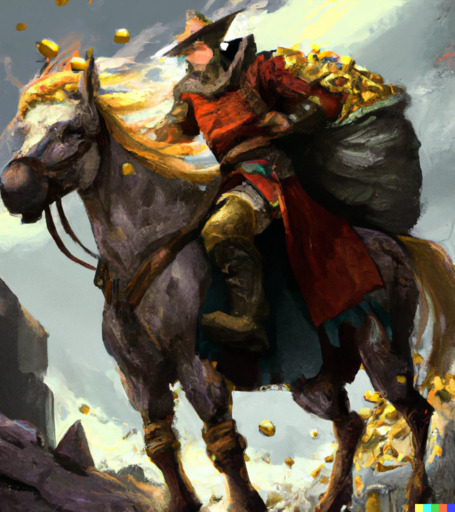
\includegraphics[width=\columnwidth]{equipment/tools goods and mounts}

        The world of Rise has a wide range of minor items like backpacks, blankets, and ten-foot poles.
        In general, the cost of those items is so insignificant from the perspective of an adventuring party that it's not worth the effort to track their cost in detail.
        A subset of particularly expensive items is included in \tref{Permanent Tools, Goods, and Mounts}.

        \subsection{Standard Adventuring Kit}
          % Technically 15.2 gp and 50.5 pounds
          A standard adventuring kit costs 10 gp, weighs 50 pounds, and contains the following items:
          \begin{itemize}
            \item Backpack
            \item Bedroll
            \item Flint and steel
            \item Rations, trail (8 days)
            \item Rope, hempen (60 ft.)
            \item Sack (empty)
            \item Tent
            \item Torch
            \item Waterskin
          \end{itemize}
      \end{longtablepreface}

      \input{generated/permanent_tools_table.tex}
  \end{longcolumn}

  \input{generated/permanent_tools.tex}
